\documentclass{article}

\def\npart{III}
\def\nyear{2018}
\def\nterm{Michaelmas}
\def\nlecturer{Professor I.\ B.\ Leader}
\def\ncourse{Combinatorics}
\def\draft{Ongoing course, rough}
\usepackage{imakeidx}
\usepackage{chngcntr}
\usepackage{marginnote}
\ifx \nauthor\undefined
  \def\nauthor{Bhavik Mehta}
\else
\fi

\author{Based on lectures by \nlecturer \\\small Notes taken by \nauthor}
\date{\nterm\ \nyear}
\title{Part \npart\ -- \ncourse}

\usepackage[utf8]{inputenc}
\usepackage{amsmath}
\usepackage{amsthm}
\usepackage{amssymb}
\usepackage{enumerate}
\usepackage{mathtools}
\usepackage{graphicx}
\usepackage[dvipsnames]{xcolor}
\usepackage{tikz}
\usepackage{wrapfig}
\usepackage{centernot}
\usepackage{float}
\usepackage{braket}
\usepackage[hypcap=true]{caption}
\usepackage{enumitem}
\usepackage[colorlinks=true, linkcolor=mblue]{hyperref}
\usepackage[nameinlink,noabbrev]{cleveref}
\usepackage{nameref}
\usepackage[margin=1.5in]{geometry}

% Theorems
\theoremstyle{definition}
\newtheorem*{aim}{Aim}
\newtheorem*{axiom}{Axiom}
\newtheorem*{claim}{Claim}
\newtheorem*{cor}{Corollary}
\newtheorem*{conjecture}{Conjecture}
\newtheorem*{defi}{Definition}
\newtheorem*{eg}{Example}
\newtheorem*{ex}{Exercise}
\newtheorem*{fact}{Fact}
\newtheorem*{law}{Law}
\newtheorem*{lemma}{Lemma}
\newtheorem*{notation}{Notation}
\newtheorem*{prop}{Proposition}
\newtheorem*{question}{Question}
\newtheorem*{rrule}{Rule}
\newtheorem*{thm}{Theorem}
\newtheorem*{assumption}{Assumption}

\newtheorem*{remark}{Remark}
\newtheorem*{warning}{Warning}
\newtheorem*{exercise}{Exercise}

% \newcommand{\nthmautorefname}{Theorem}

\newtheorem{nthm}{Theorem}[section]
\newtheorem{nlemma}[nthm]{Lemma}
\newtheorem{nprop}[nthm]{Proposition}
\newtheorem{ncor}[nthm]{Corollary}
\newtheorem{ndef}[nthm]{Definition}

% Special sets
\newcommand{\C}{\mathbb{C}}
\newcommand{\N}{\mathbb{N}}
\newcommand{\Q}{\mathbb{Q}}
\newcommand{\R}{\mathbb{R}}
\newcommand{\Z}{\mathbb{Z}}

\newcommand{\abs}[1]{\left\lvert #1\right\rvert}
\newcommand{\norm}[1]{\left\lVert #1\right\rVert}
\renewcommand{\vec}[1]{\boldsymbol{\mathbf{#1}}}

\let\Im\relax
\let\Re\relax

\DeclareMathOperator{\Im}{Im}
\DeclareMathOperator{\Re}{Re}
\DeclareMathOperator{\id}{id}

\definecolor{mblue}{rgb}{0., 0.05, 0.6}

\usepackage{pgfplots}
\makeindex[intoc]
\usetikzlibrary{fadings, decorations.pathmorphing, shadings}
%\pagecolor{black}

% preamble

\setcounter{section}{-1}
% \counterwithout{nthm}{section}

\reversemarginpar

\DeclarePairedDelimiter\ceil{\lceil}{\rceil}
\DeclarePairedDelimiter\floor{\lfloor}{\rfloor}
\DeclareMathOperator\tr{tr}

\tikzset{
    dot/.style={fill=black, circle, inner sep=1pt}
}

\newcommand{\sym}{\bigtriangleup}

\newcommand{\ihalf}[1]{\floor{\frac{#1}{2}}}
\newcommand{\ihalfc}[1]{\ceil{\frac{#1}{2}}}
\newcommand{\A}{\mathcal{A}}
\newcommand{\named}[1]{\textbf{#1}\index{#1}}

%\newtheorem{manualtheoreminner}{Theorem}
%\newenvironment{manualtheorem}[1]{%
%    \renewcommand\themanualtheoreminner{#1}%
%    \manualtheoreminner
%}{\endmanualtheoreminner}

% and here we go!

\let\oldsubset\subset
\let\subset\subseteq

\begin{document}
%\color{white}
\maketitle

\tableofcontents

\clearpage
\section{Introduction}
\marginnote{\emph{Lecture 1}}[0cm]
Combinatorics tends to have problems which are easy to state and hard to prove.
One of the reasons for this is that it is often unclear where to start - for instance in linear algebra we can often start by picking a basis.
Proofs tend to have the property that they seem to take thousands of years to come up with, and a single line to write down.
In this course, we learn some techniques which make problems sounding very hard become very easy.

We start with set systems, which builds on the idea of subsets and containment.
Next, we study isoperimetric inequalities.
In the continuous case, in the plane, a typical problem is to find the maximum area one can enclose with a fixed perimeter, which is solved by a circle.
Similarly, a soap bubble will minimise its surface area for a fixed volume.
Here, in the discrete case, we will try to understand `how tightly' we can pack subsets.
Finally, we look at continuous projections.
For instance, given a subset of space, suppose we know the $z$-coordinate of all points is between $0$ and $1$, and the projection to the $xy$-plane has area $A$, we know the total volume is bounded by $A$.
We generalise this result into higher dimensions and the box result, which has applications in combinatorics.

While all examinable proofs will be included in lectures, relevant books for this course are:
\begin{enumerate}
  \item \emph{Combinatorics}, Bollob\'{a}s, C.U.P., 1996. This matches chapter 1 excellently and parts of chapter 2. It is a gentle read and includes other developments in combinatorics.
  \item \emph{Combinatorics of finite sets}, Anderson, O.U.P., 1987. It is a simple and clear study on chapter 1.
\end{enumerate}

\clearpage
\section{Set systems}
\begin{defi}[Set system]\index{set system}\hypertarget{def:ss}
  Let $X$ be a set. A \named{set system} on $X$ (or \named{family of subsets} of $X$) is a family $\mathcal{A} \subseteq \mathcal{P}(X)$.
\end{defi}
For instance, we write \hypertarget{def:superr}$X^{(r)} = \set{A \subset X | |A| = r}$, so $X^{(r)}$ is a \hyperlink{def:ss}{set system} on $X$.
Unless otherwise stated,
\begin{equation*}
  \hypertarget{def:ints}X = [n] \coloneqq \{1,2,\dotsc,n\},
\end{equation*}
e.g.\ $|X^{\hyperlink{def:superr}{(r)}}| = \binom{n}{r}$.
Thus $\hyperlink{def:ints}{[4]}^{(2)} = \{12,13,14,23,24,34\}$, so $|[4]^{(2)}| = 6$.

Often, we make $\mathcal{P}(X)$ into a graph, called $Q_n$, by joining $A$ to $B$ if $|A \sym B| = 1$, i.e.\ if $A = B \cup \{i\}$ for some $i \notin B$ (or vice versa).
For instance, here is a picture of $Q_3$:
\begin{center}
  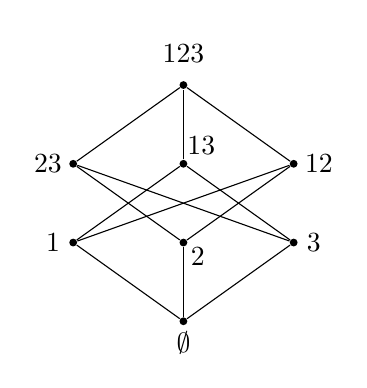
\begin{tikzpicture}[xscale=1.4, every node/.style={fill=black, circle, inner sep=1pt}]
    \node [label=below:$\emptyset$] (empty) at (0,0) {};
    \node [label=left:$1$] (1) at (-1,1) {};
    \node [label=below right:$2$] (2) at (0,1) {};
    \node [label=right:$3$] (3) at (1,1) {};
    \node [label=left:$23$] (23) at (-1,2) {};
    \node [label=above right:$13$] (13) at (0,2) {};
    \node [label=right:$12$] (12) at (1,2) {};
    \node [label=above:$123$] (123) at (0,3) {};
    \draw (empty) -- (1);
    \draw (empty) -- (2);
    \draw (empty) -- (3);
    \draw (1) -- (12);
    \draw (1) -- (13);
    \draw (2) -- (12);
    \draw (2) -- (23);
    \draw (3) -- (13);
    \draw (3) -- (23);
    \draw (12) -- (123);
    \draw (13) -- (123);
    \draw (23) -- (123);
  \end{tikzpicture}
\end{center}

As we know, the picture gets `thicker' in the middle. But, for odd $n$, is it not clear where exactly the middle is, so in the odd case we have two equally sized large blobs in the middle.

\begin{center}
  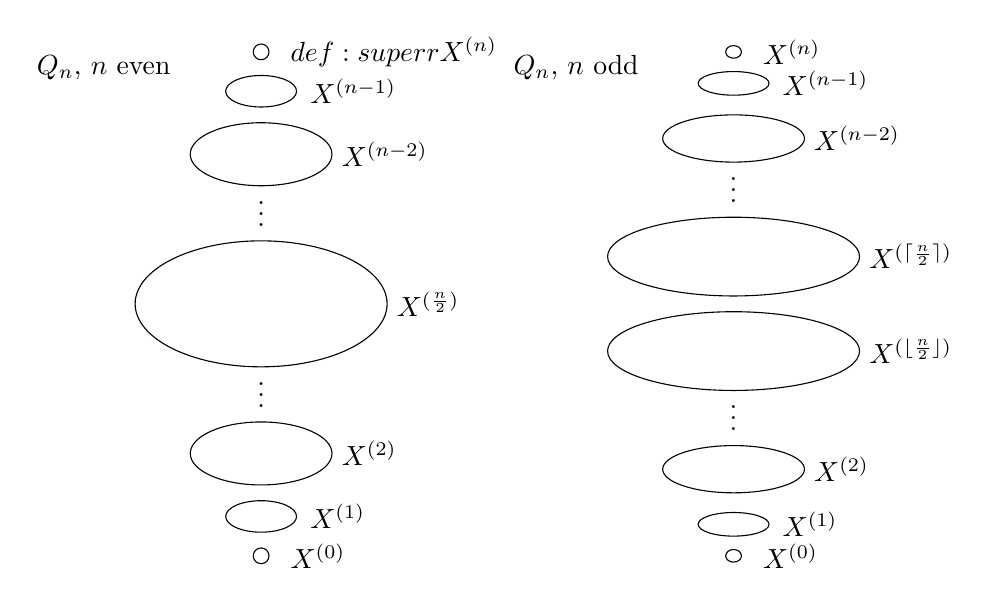
\begin{tikzpicture}
    \begin{scope}
      \node at (-2, 3) {$Q_n$, $n$ even};

      \draw (0,3.2) circle [x radius=1mm, y radius=1mm];
      \node [right] at (0.25, 3.2) {$\hyperlink{def:superr}{X^{(n)}}$};

      \draw (0,2.7) circle [x radius=4.5mm, y radius=2mm];
      \node [right] at (0.5, 2.7) {$X^{(n-1)}$};

      \draw (0,1.9) circle [x radius=9mm, y radius=4mm];
      \node [right] at (0.9, 1.9) {$X^{(n-2)}$};

      \node at (0,1.25) {$\vdots$};

      \draw (0,0) circle [x radius=16mm, y radius=8mm];
      \node [right] at (1.6, 0) {$X^{(\frac{n}{2})}$};

      \node at (0,-1.05) {$\vdots$};

      \draw (0,-1.9) circle [x radius=9mm, y radius=4mm];
      \node [right] at (0.9, -1.9) {$X^{(2)}$};

      \draw (0,-2.7) circle [x radius=4.5mm, y radius=2mm];
      \node [right] at (0.5, -2.7) {$X^{(1)}$};

      \draw (0,-3.2) circle [x radius=1mm, y radius=1mm];
      \node [right] at (0.25, -3.2) {$X^{(0)}$};
    \end{scope}

    \begin{scope}[xshift=6cm]
      \node at (-2, 3) {$Q_n$, $n$ odd};

      \draw (0,3.2) circle [x radius=1mm, y radius=0.8mm];
      \node [right] at (0.25, 3.2) {$X^{(n)}$};

      \draw (0,2.8) circle [x radius=4.5mm, y radius=1.5mm];
      \node [right] at (0.5, 2.8) {$X^{(n-1)}$};

      \draw (0,2.1) circle [x radius=9mm, y radius=3mm];
      \node [right] at (0.9, 2.1) {$X^{(n-2)}$};

      \node at (0,1.55) {$\vdots$};

      \draw (0,0.6) circle [x radius=16mm, y radius=5mm];
      \node [right] at (1.6, 0.6) {$X^{(\ceil{\frac{n}{2}})}$};

      \draw (0,-0.6) circle [x radius=16mm, y radius=5mm];
      \node [right] at (1.6, -0.6) {$X^{(\floor{\frac{n}{2}})}$};

      \node at (0,-1.35) {$\vdots$};

      \draw (0,-2.1) circle [x radius=9mm, y radius=3mm];
      \node [right] at (0.9, -2.1) {$X^{(2)}$};

      \draw (0,-2.8) circle [x radius=4.5mm, y radius=1.5mm];
      \node [right] at (0.5, -2.8) {$X^{(1)}$};

      \draw (0,-3.2) circle [x radius=1mm, y radius=0.8mm];
      \node [right] at (0.25, -3.2) {$X^{(0)}$};
    \end{scope}
  \end{tikzpicture}
\end{center}

If we identify a set $A \subseteq X$ with a $0$-$1$ sequence of length $n$, e.g.\ $134 \longleftrightarrow 1011000\dots0$, via $A \longleftrightarrow 1_{A}$ or $\chi_A$, the characteristic function,
then $Q_3$ looks like
\begin{center}
  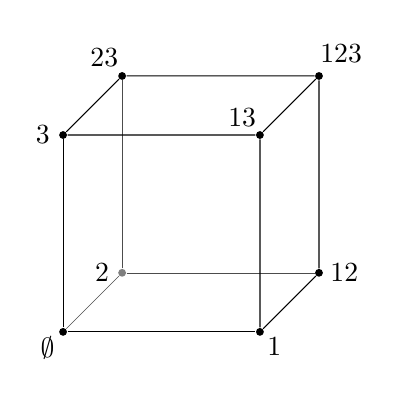
\begin{tikzpicture}[every node/.style={fill=black, circle, inner sep=1pt}, scale=2.5]
    \node [label=below left:$\emptyset$] (empty) at (0,0) {};
    \node [label=below right:$1$] (1) at (1, 0) {};
    \node [fill opacity=0.5, label=left:$2$] (2) at (0.3,0.3) {};
    \node [label=left:$3$] (3) at (0, 1) {};
    \node [label=above left:$13$] (13) at (1, 1) {};
    \node [label=right:$12$] (12) at (1.3, 0.3) {};
    \node [label=above left:$23$] (23) at (0.3, 1.3) {};
    \node [label=above right:$123$] (123) at (1.3, 1.3) {};
    \draw (empty) -- (1);
    \draw [opacity=0.7, very thin] (empty) -- (2);
    \draw (empty) -- (3);
    \draw (1) -- (12);
    \draw (1) -- (13);
    \draw [opacity=0.7, very thin] (2) -- (12);
    \draw [opacity=0.7, very thin] (2) -- (23);
    \draw (3) -- (13);
    \draw (3) -- (23);
    \draw (12) -- (123);
    \draw (13) -- (123);
    \draw (23) -- (123);
  \end{tikzpicture}
\end{center}
\begin{defi}[Hypercube]\index{hypercube}\hypertarget{def:qn}
  $Q_n$ is often called the \named{hypercube} or \textbf{discrete cube} or \textbf{$n$-cube}.
\end{defi}
It is important to keep \emph{both} these pictures in mind: for induction the cube image is more instructive, but when thinking about layers the earlier image is more helpful.

\subsection{Chains and antichains}
\begin{defi}[Chain]\index{chain}\hypertarget{def:chain}
  A family $\mathcal{A} \subseteq \mathcal{P}(X)$ is a \named{chain} if $\forall A, B \in \mathcal{A}$, we have $A \subseteq B$ or $B \subseteq A$.
\end{defi}
\begin{defi}[Antichain]\index{antichain}\hypertarget{def:antichain}
  A family $\mathcal{A} \subseteq \mathcal{P}(X)$ is an \named{antichain} if $\forall A,B \in \mathcal{A}$ with $A \neq B \Rightarrow A \nsubseteq B$.
\end{defi}
\begin{eg}
  For instance, $\{12, 125, 123589\}$ is an \hyperlink{def:chain}{chain}, and $\{1,467,2456\}$ is an \hyperlink{def:antichain}{antichain}.
\end{eg}

In this course, we ask questions like, how large can a \hyperlink{def:chain}{chain} be?
We can achieve $|\mathcal{A}| = n+1$, e.g.\ $\{\emptyset, 1, 12, 123, \dotsc, [n]\}$.
It is easy to visualise this by picking `one per level':
\begin{center}
  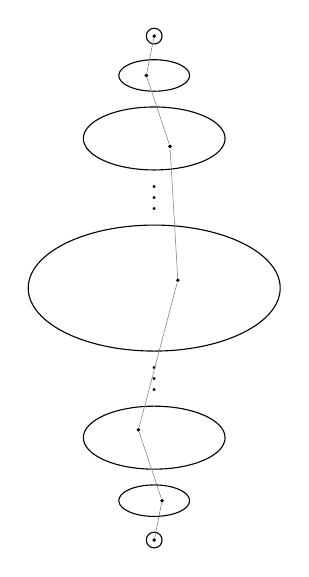
\begin{tikzpicture}
      \draw (0,3.2) circle [x radius=1mm, y radius=1mm];
      \draw (0,2.7) circle [x radius=4.5mm, y radius=2mm];
      \draw (0,1.9) circle [x radius=9mm, y radius=4mm];
      \node at (0,1.25) {$\vdots$};
      \draw (0,0) circle [x radius=16mm, y radius=8mm];
      \node at (0,-1.05) {$\vdots$};
      \draw (0,-1.9) circle [x radius=9mm, y radius=4mm];
      \draw (0,-2.7) circle [x radius=4.5mm, y radius=2mm];
      \draw (0,-3.2) circle [x radius=1mm, y radius=1mm];
      \begin{scope}[every node/.style={fill=black, circle, inner sep=0.5pt}]
        \node (0) at (0,-3.2)    {};
        \node (1) at (0.1,-2.7)  {};
        \node (2) at (-0.2,-1.8) {};
        \node (3) at (0.3, 0.1)   {};
        \node (4) at (0.2,1.8)   {};
        \node (5) at (-0.1,2.7)  {};
        \node (6) at (0,3.2)     {};
        \draw[very thin, gray] (0) -- (1) -- (2) -- (3) -- (4) -- (5) -- (6);
      \end{scope}
  \end{tikzpicture}
\end{center}

We cannot exceed $n+1$, since a chain must meet each `level' $X^{(r)}$ ($0 \leq r \leq n$) in at most one place.

How large can an \hyperlink{def:antichain}{antichain} be?
We could achieve $\mathcal{A}=n$, e.g.\ $\mathcal{A} = \{1,2,3,\dotsc,n\}$ (and this is maximal).
Indeed, we could take $\mathcal{A} = X^{(r)}$ for any $r$, so we can achieve $|\mathcal{A}| = \binom{n}{\floor{\frac{n}{2}}}$.
Can we beat this?
Aim: Prove this is the winner.

\marginnote{\emph{Lecture 2}}[0cm]
Inspired by `each \hyperlink{def:chain}{chain} meets each level $X^{(r)}$ in at most one place' for chains, we try to decompose $\hyperlink{def:qn}{Q_n}$ into chains to find large \hyperlink{def:antichain}{antichains}.
\begin{nthm}[Sperner's Lemma]\label{thm:sperner1}\index{Sperner's Lemma}
  Let $\mathcal{A} \subseteq \mathcal{P}(X)$ be an \hyperlink{def:antichain}{antichain}.
  Then $|\mathcal{A}| \leq \binom{n}{\floor{\frac{n}{2}}}$.
\end{nthm}
\begin{proof}
  It is sufficient to partition $\mathcal{P}(X)$ into $\binom{n}{\floor{\frac{n}{2}}}$ \hyperlink{def:chain}{chains}.
  For this, it is sufficient to show
  \begin{enumerate}[label=(\roman*)]
    \item $\forall r < \frac{n}{2}$, there is a matching from \hyperlink{def:superr}{$X^{(r)}$} to $X^{(r+1)}$
    \item $\forall r > \frac{n}{2}$, there is a matching from $X^{(r)}$ to $X^{(r-1)}$.
  \end{enumerate}
  Then put these matchings together to form chains, each passing through $X^{(\floor{\frac{n}{2}})}$, so there are $\binom{n}{\floor{\frac{n}{2}}}$ of them. (Recall we have a \hyperlink{def:ints}{natural graph structure} on \hyperlink{def:qn}{$Q_n$})

  \begin{center}
    \begin{tikzpicture}
        \tikzfading[name=fade up, bottom color=transparent!0,
          top color=transparent!100]
        \tikzfading[name=fade down, bottom color=transparent!100,
          top color=transparent!0]
        \draw (0,3.2) circle [x radius=1mm, y radius=1mm];
        \node [right] at (0.25, 3.2) {$X^{(n)}$};

        \draw (0,2.7) circle [x radius=4.5mm, y radius=2mm];
        \node [right] at (0.5, 2.7) {$X^{(n-1)}$};

        \draw (0,1.9) circle [x radius=9mm, y radius=4mm];
        \node [right] at (0.9, 1.9) {$X^{(n-2)}$};

        \draw [bblue] (0,3.2) -- (0,2.7) -- (0,1.9);
        \draw [bblue, path fading=fade down] (0,1.9) -- (0,1.4);

        \draw [bblue] (0.2,2.7) to[out=270, in=100] (0.25,1.9);
        \draw [bblue, path fading=fade down] (0.25,1.9) to[out=-80, in=110] (0.4, 1.4);

        \draw [bblue] (-0.2,2.7) to[out=270, in=80] (-0.25,1.9);
        \draw [bblue, path fading=fade down] (-0.25,1.9) to[out=-100, in=70] (-0.4, 1.4);

        \draw [bblue, path fading=fade down] (0.5, 1.9) -- (0.7, 1.4);
        \draw [bblue, path fading=fade down] (-0.5, 1.9) -- (-0.7, 1.4);

        \node at (0,1.25) {$\vdots$};

        \foreach \val in {-1.4,-1.0,...,1.4} {
          \draw [bblue, path fading=fade up] (\val*0.8,1) to[in=90,out=270] (\val,0); % -- (\val*0.8,-1);
          \draw [bblue, path fading=fade down] (\val*0.8,-1) to[in=270,out=90] (\val,0);
        }

        \draw (0,0) circle [x radius=16mm, y radius=8mm];
        \node [right] at (1.6, 0) {$X^{(\floor{\frac{n}{2}})}$};

        \node at (0,-1.05) {$\vdots$};

        \begin{scope}[yscale=-1]
          \draw (0,3.2) circle [x radius=1mm, y radius=1mm];
          \node [right] at (0.25, 3.2) {$X^{(0)}$};

          \draw (0,2.7) circle [x radius=4.5mm, y radius=2mm];
          \node [right] at (0.5, 2.7) {$X^{(1)}$};

          \draw (0,1.9) circle [x radius=9mm, y radius=4mm];
          \node [right] at (0.9, 1.9) {$X^{(2)}$};

          \draw [bblue] (0,3.2) -- (0,2.7) -- (0,1.9);
          \draw [bblue, path fading=fade up] (0,1.9) -- (0,1.4);

          \draw [bblue] (0.2,2.7) to[out=270, in=100] (0.25,1.9);
          \draw [bblue, path fading=fade up] (0.25,1.9) to[out=-80, in=110] (0.4, 1.4);

          \draw [bblue] (-0.2,2.7) to[out=270, in=80] (-0.25,1.9);
          \draw [bblue, path fading=fade up] (-0.25,1.9) to[out=-100, in=70] (-0.4, 1.4);

          \draw [bblue, path fading=fade up] (0.5, 1.9) -- (0.7, 1.4);
          \draw [bblue, path fading=fade up] (-0.5, 1.9) -- (-0.7, 1.4);
        \end{scope}
    \end{tikzpicture}
  \end{center}

  By taking complements, it is sufficient to prove (i).

  Consider the subgraph of \hyperlink{def:qn}{$Q_n$} spanned by $\hyperlink{def:superr}{X^{(r)}} \cup X^{(r+1)}$. It is bipartite.
  For any $\mathcal{B} \subseteq X^{(r)}$, we have that
  \begin{itemize}
    \item The number of edges from $\mathcal{B}$ to $\Gamma(\mathcal{B})$ is $|\mathcal{B}| (n-r)$ (each point in $X^{(r)}$ has degree $n-r$).
    \item The number of edges from $\mathcal{B}$ to $\Gamma(\mathcal{B})$ is at most $|\Gamma(\mathcal{B})| (r+1)$ (each point in $X^{(r+1)}$ has degree $r+1$).
  \end{itemize}
  \begin{center}
    \begin{tikzpicture}
      \draw (0,1) circle [x radius=1.7cm, y radius=0.9cm];
      \node [right] at (1.7, 1) {$X^{(r+1)}$};
      \node [left, bred] at (0.1, 1.1) {$\Gamma(\mathcal{B})$};

      \draw (0, -1) circle [x radius=1.2cm, y radius=0.6cm];
      \node [right] at (1.2, -1) {$X^{(r)}$};
      \node [left, bred] at (0.3, -0.9) {$\mathcal{B}$};

      \begin{scope}[every path/.style={decorate, decoration={random steps, segment length=1.5pt, amplitude=0.7pt}, bred, fill=bred!20}]
        \draw (0.6, -0.9) circle [x radius=0.3cm, y radius=0.25cm];
        \draw (0.7, 1.1) circle [x radius=0.6cm, y radius=0.45cm];
      \end{scope}
      %\foreach \x in {0.4,0.5,...,1.1} {
      %  \draw [very thin] (\x,1.1) to (\x*0.6+0.2,-0.9);
      %}
    \end{tikzpicture}
  \end{center}
  Thus
  \begin{align*}
    |\Gamma(\mathcal{B})| &\geq |\mathcal{B}| \frac{n-r}{r+1} \\
                               &\geq |\mathcal{B}|
  \end{align*}
  as $r < \frac{n}{2}$.
  Hence by Hall's theorem, there is a matching.
\end{proof}

\begin{remark}
  Recall $\binom{n}{\floor{\frac{n}{2}}}$ was achievable, for example $\mathcal{A} = \hyperlink{def:superr}{X^{(\floor{\frac{n}{2}})}}$.
  This proof says nothing about extremal cases - which \hyperlink{def:antichain}{antichains} have size $\binom{n}{\floor{\frac{n}{2}}}$?
\end{remark}

Aim: For $\mathcal{A}$ an antichain,
\begin{equation*}
  \sum_{r=0}^n \frac{|\mathcal{A} \cap X^{(r)}|}{\binom{n}{r}} \leq 1.
\end{equation*}
This trivially implies \nameref{thm:sperner1}.

\begin{defi}[Shadow]\index{shadow}\hypertarget{def:shadow}
  Let $\mathcal{A} \subseteq X^{(r)}$, for some $1 \leq r \leq n$.
  The \named{shadow} or \named{corner shadow} of $\mathcal{A}$ is
  \begin{equation*}
    \partial \mathcal{A} \equiv \partial^- \mathcal{A} \coloneqq \set{A - \{i\} | A \in \mathcal{A},\; i \in A}
  \end{equation*}
  so $\partial \mathcal{A} \subset X^{(r-1)}$.
\end{defi}
\begin{center}
  \begin{tikzpicture}
    \draw [bgreen, opacity=0.8] (0.2,1.1) -- (0.2,-1);
    \draw [bgreen, opacity=0.8] (1.2,1.1) -- (1,-1);

    \draw (0,1) circle [x radius=1.7cm, y radius=0.9cm];
    \node [right] at (1.7, 1) {$X^{(r)}$};
    \node [left, bgreen] at (0.2, 1.1) {$A$};

    \draw (0, -1) circle [x radius=1.2cm, y radius=0.6cm];
    \node [right] at (1.2, -1) {$X^{(r-1)}$};
    \node [left, bgreen] at (0.2, -1) {$\partial A$};
    \begin{scope}[every path/.style={decorate, decoration={random steps, segment length=1.5pt, amplitude=0.7pt}, bgreen, fill=bgreen!20}]
      \draw (0.6, -1) circle [x radius=0.4cm, y radius=0.3cm];
      \draw (0.7, 1.1) circle [x radius=0.5cm, y radius=0.4cm];
    \end{scope}
  \end{tikzpicture}
\end{center}
For example, if $\mathcal{A} = \{123,124,134,135\} \subset X^{(3)}$, then
\begin{equation*}\hyperlink{def:shadow}{\partial \mathcal{A}} = \{12,13,23,24,34,15,35\} \subset X^{(2)}.\end{equation*}

\begin{nlemma}[Local LYM]\label{thm:locallym2}\index{Local LYM}
  Let $\mathcal{A} \subseteq \hyperlink{def:superr}{X^{(r)}}$, $1 \leq r \leq n$. Then
  \begin{equation*}
    \frac{|\hyperlink{def:shadow}{\partial \mathcal{A}}|}{\binom{n}{r-1}} \geq \frac{|\mathcal{A}|}{\binom{n}{r}}.
  \end{equation*}
  `The fraction of the layer occupied increases when we take the \hyperlink{def:shadow}{shadow}'.
\end{nlemma}
\begin{proof}
  Counting from above, there are $r|\mathcal{A}|$ edges $\mathcal{A}$ to $\hyperlink{def:shadow}{\partial \mathcal{A}}$.
  Counting from below, the number of edges $\mathcal{A}$ to $\partial \mathcal{A}$ is at most $(n-r+1) |\partial \mathcal{A}|$, so
  \begin{equation*}
    \frac{|\partial \mathcal{A}|}{|\mathcal{A}|} \geq \frac{r}{n-r+1}.
  \end{equation*}
  But
  \begin{equation*}
    \frac{\binom{n}{r-1}}{\binom{n}{r}} = \frac{r}{n-r+1}.\qedhere
  \end{equation*}
\end{proof}

When do we get equality in \nameref{thm:locallym2}? We'd need $(A - \{i\}) \cup \{j\} \in \mathcal{A}\;\;\forall A \in \mathcal{A},\; i \in A,\; j \notin A$. Hence $\mathcal{A} = X^{r}$ or $\emptyset$.

The LYM in \nameref{thm:locallym2} stands for `Lubell–Yamamoto–Meshalkin'.
We can use \nameref{thm:locallym2} to prove:
\begin{nthm}[LYM]\label{thm:lym3}\index{LYM}
  Let $\mathcal{A} \subset \mathcal{P}(X)$ be an \hyperlink{def:antichain}{antichain}.
  Then
  \begin{equation*}
    \sum_{r=0}^n \frac{|\mathcal{A} \cap \hyperlink{def:superr}{X^{(r)}}|}{\binom{n}{r}} \leq 1.
  \end{equation*}
\end{nthm}
\begin{proof}[Proof 1: `Bubble down with \nameref{thm:locallym2}']
  Write $\mathcal{A}_r = \mathcal{A} \cap X^{(r)}$.
  We have $\frac{|\mathcal{A}_n|}{\binom{n}{n}} \leq 1$.
  Also, $\hyperlink{def:shadow}{\partial \mathcal{A}_n}$ and $\mathcal{A}_{n-1}$ are distinct since $\mathcal{A}$ was an \hyperlink{def:antichain}{antichain}, so
  \begin{align*}
    \frac{|\partial A_n|}{\binom{n}{n-1}} + \frac{|A_{n-1}|}{\binom{n}{n-1}} &= \frac{|\partial A_n \cup A_{n-1}|}{\binom{n}{n-1}} \\
    \implies \frac{|A_n|}{\binom{n}{n}} + \frac{|\mathcal{A}_{n-1}|}{\binom{n}{n-1}} &\leq 1
  \end{align*}
  by \nameref{thm:locallym2}.

  Also, $\partial(\partial \mathcal{A}_n \cup \mathcal{A}_{n-1})$ is disjoint from $\mathcal{A}_{n-2}$, again since $\mathcal{A}$ is an antichain so
  \begin{align*}
    \frac{|\partial(\partial \mathcal{A}_n \cup \mathcal{A}_{n-1})|}{\binom{n}{n-2}} + \frac{\mathcal{A}_{n-2}}{{n \choose n-2}} &\leq 1, \\
    \implies \frac{|(\partial \mathcal{A}_n \cup \mathcal{A}_{n-1})|}{\binom{n}{n-1}} + \frac{\mathcal{A}_{n-2}}{{n \choose n-2}} &\leq 1, \\
    \implies \frac{\mathcal{A}_n}{\binom{n}{n}} + \frac{\mathcal{A}_{n-1}}{\binom{n}{n-1}} + \frac{\mathcal{A}_{n-2}}{\binom{n}{n-2}} &\leq 1.
  \end{align*}
  \begin{center}
    \begin{tikzpicture}[scale=2]
      \draw (0, 1) circle [x radius=0.5cm, y radius=0.3cm];
      \draw (0, 0) circle [x radius=0.9cm, y radius=0.5cm];
      \draw (0,-1.6) circle [x radius=1.4cm, y radius=0.8cm];

      \draw [bred, opacity=0.8] (-0.3, 1) -- (-0.6,0) -- (-0.1,-1.6);
      \draw [bred, opacity=0.8] (0.1, 1) -- (0,0);
      \draw [bred, opacity=0.8] (0.65,0) -- (0.9,-1.6);

      \node [bred] at (0.3,1) {$\mathcal{A}_n$};
      \node [bred] at (-0.3,-0.3) {$\partial \mathcal{A}_n$};
      \node [bred] at (0.3,-0.3) {$\mathcal{A}_{n-1}$};
      \node [bred] at (-0.7,-1.9) {$\mathcal{A}_{n-2}$};
      \node [bred] at (0.3,-2.1) {$\partial(\partial A_n \cup A_{n-1})$};

      \begin{scope}[every path/.style={decorate, decoration={random steps, segment length=1.5pt, amplitude=0.7pt}, bred, fill=bred!20}]
        \draw [thick] (-0.1, 1) circle [x radius=0.2 cm, y radius=1.5 mm];
        \draw [fill=bred!10] (-0.3, 0) circle [x radius=0.3 cm, y radius=0.2 cm];
        \draw [thick] (0.4, 0) circle [x radius=0.25 cm, y radius=0.2 cm];
        \draw [thick] (-0.7, -1.5) circle [x radius=0.3cm, y radius=0.25cm];
        \draw [fill=bred!10] (0.4, -1.6) circle [x radius=0.5cm, y radius=0.35cm];
      \end{scope}
    \end{tikzpicture}
  \end{center}
  Keep going, we obtain
  \begin{equation*}
    \frac{\mathcal{A}_n}{\binom{n}{n}} + \frac{\mathcal{A}_{n-1}}{\binom{n}{n-1}} + \dotsm + \frac{\mathcal{A}_0}{\binom{n}{0}} \leq 1. \qedhere
  \end{equation*}
\end{proof}

When do we get equality in \nameref{thm:lym3}?
We must have had equality in each use of \nameref{thm:locallym2}.
So the first (greatest) $r$ with $\mathcal{A}_r \neq \emptyset$ must have $\mathcal{A}_r = X^{(r)}$ thus $\mathcal{\mathcal{A}} = X^{(r)}$.
Hence equality in \nameref{thm:sperner1} $\iff$ $\mathcal{A} = X^{(\frac{n}{2})}$ for $n$ even and $\mathcal{A} = X^{(\ihalf{n})}$ or $X^{(\ihalfc{n})}$ for $n$ odd.

\marginnote{\emph{Lecture 3}}[0cm]
\begin{proof}[Proof 2]
  Choose uniformly at random a maximal \hyperlink{def:chain}{chain} $\mathcal{C}$ (i.e.\ $\mathcal{C}_0 \subset \mathcal{C}_1 \subset \mathcal{C}_2 \subset \dotsb \subset \mathcal{C}_n$) with $|\mathcal{C}_i| = i \; \forall i$.
  For a given \hyperlink{def:superr}{$r$-set} $A$,
 \begin{align*}\mathbb{P}(A \in \mathcal{C}) = &\frac{1}{\binom{n}{r}} \qquad \qquad \text{(all $r$-sets are equally likely)} \\
    \mathbb{P}(\mathcal{A}_r \text{ meets } \mathcal{C}) = &\frac{|\mathcal{A}_r|}{\binom{n}{r}} \qquad \qquad \text{(events are disjoint)} \\
    \implies \mathbb{P}(\mathcal{A} \text{ meets }\mathcal{C}) = &\sum_{r=0}^n \frac{|\mathcal{A}_r|}{\binom{n}{r}}. \\
    \implies &\sum_{i=0}^n \frac{|\mathcal{A}_r|}{\binom{n}{r}} \leq 1. \qedhere
  \end{align*}
\end{proof}
\begin{remark}
  Equivalently, the number of maximal chains is $n!$, and the number containing a given $r$-set is $r! (n-r)!$, so $\sum |\mathcal{A}_r| r! (n-r)! \leq n!$.
\end{remark}
\subsection{Shadows}
For $\mathcal{A} \subset X^{(r)}$, we know $|\partial A| \geq |A| \frac{r}{n-r+1}$ - but equality is rare (only for $\mathcal{A} = \emptyset$ or $\mathcal{A} = X^{(r)}$).

Given $|\mathcal{A}|$, how should we choose $\mathcal{A} \subset X^{(r)}$ to minimise $|\partial A|$?
(Ultimately, we are asking `how tightly can we pack some $r$-sets?')
If $|\mathcal{A}| = \binom{k}{r}$, it is believable that we'd take $\mathcal{A} = [k]^{(r)}$ - giving $\partial \mathcal{A} = [k]^{(r-1)}$.
What if $\binom{k}{r} < |\mathcal{A}| < \binom{k+1}{r}$? Believable that we'd take $[k]^{(r)}$ and some other $r$-sets from $[k+1]^{(r)}$.
For instance, if $\mathcal{A} \subset X^{(3)}$ with $|\mathcal{A}| = \binom{7}{3} + \binom{4}{2}$, we'd take $\mathcal{A} = [7]^{(3)} \cup \set{A \cup \{8\} | A\in [4]^{(2)}}$

\subsubsection{Two total orderings on \texorpdfstring{$X^{(r)}$}{X(r)}}
Given $A,B \in \hyperlink{def:superr}{X^{(r)}}$, say $A = a_1 \dotsb a_r$, $B = b_1 \dotsb b_r$.
\begin{defi}[Lexicographic order]\index{lexicographic order}\hypertarget{def:lex}
  Say $A < B$ in the \named{lexicographic order} or \textbf{lex order} if for some $i$ we have $a_i < b_i$ and $a_j = b_j \; \forall j < i$.
\end{defi}
Equivalently, $a_i < b_i$, where $i = \min\set{j | a_j \neq b_j}$.
`Use small numbers', dictionary order.

\begin{eg}\leavevmode
  \begin{itemize}
    \item The \hyperlink{def:lex}{lex order} on $\hyperlink{def:ints}{[4]}^{\hyperlink{def:superr}{(2)}}$ is
      \begin{equation*}
        12,13,14,23,24,34.
      \end{equation*}
    \item The lex order on $[6]^{(3)}$ is
      \begin{align*}
        &123,124,125,126,134,135,136,145,146,156,\\
        &234,235,236,245,246,256,345,346,356,456.
      \end{align*}
  \end{itemize}
\end{eg}

\begin{defi}[Colexicographic order]\index{colexicographic order}\hypertarget{def:colex}
  Say $A < B$ in the \named{colexicographic order} or \textbf{colex order} if for some $i$ have $a_i < b_i$ and $a_j = b_j \; \forall j > i$.
\end{defi}
Equivalently, $a_i < b_i$ where $i = \max\set{j | a_j \neq b_j}$.
`Avoid large numbers'. Equivalently, $A < B$ if $\sum_{i \in A} 2^i < \sum_{i \in B} 2^i$.
\begin{eg}\leavevmode
  \begin{itemize}
    \item \hyperlink{def:colex}{Colex} on $\hyperlink{def:ints}{[4]}^{\hyperlink{def:superr}{(2)}}$ is
      \begin{equation*}
        12,13,23,14,24,34
      \end{equation*}
    \item Colex on $[6]^{(3)}$ is
      \begin{align*}
        &123,124,134,234,125,135,235,145,245,345,\\
        &126,136,236,146,246,346,156,256,356,456.
      \end{align*}
  \end{itemize}
\end{eg}
Note: In \hyperlink{def:colex}{colex}, $\hyperlink{def:ints}{[k]}^{\hyperlink{def:superr}{(r)}}$ is an initial segment of $[k+1]^{(r+1)}$, so we could view colex as an enumeration of $\mathbb{N}^{(r)}$ (but this is false for \hyperlink{def:lex}{lex}).

\begin{aim}
  Initial segments of \hyperlink{def:colex}{colex} minimise $\hyperlink{def:shadow}{\partial}$, i.e.\ if $\mathcal{A} \subset \hyperlink{def:superr}{X^{(r)}}$ and $\mathcal{C} \subset X^{(r)}$ is the first $|\mathcal{A}|$ $r$-sets in \hyperlink{def:colex}{colex}, then $|\partial \mathcal{A}| \geq |\partial \mathcal{C}|$.
\end{aim}
This is known as the Kruskal-Katona theorem.
In particular, \begin{equation*}|\mathcal{A}| = \binom{k}{r} \implies |\partial A| \geq \binom{k}{r-1}.\end{equation*}

\subsection{Compressions}
\begin{idea}
We want to `replace' $\mathcal{A} \subset X^{(r)}$ with some $\mathcal{A}' \subset X^{(r)}$ such that
\begin{enumerate}[label=(\roman*)]
  \item $|\mathcal{A}'| = |\mathcal{A}|$
  \item $|\hyperlink{def:shadow}{\partial \mathcal{A}'}| \leq |\partial \mathcal{A}|$
  \item $\mathcal{A}'$ `looks more like $\mathcal{C}$' than $\mathcal{A}$ did.
\end{enumerate}
Ideally, we'd compress $\mathcal{A} \to \mathcal{A}' \to \mathcal{A}'' \to \dotsm \to \mathcal{B}$ where either $\mathcal{B} = \mathcal{C}$ or $\mathcal{B}$ is so similar to $\mathcal{C}$ that we can see directly that $|\partial \mathcal{B}| \geq |\partial \mathcal{C}|$.
\end{idea}

\marginnote{\emph{Lecture 4}}[0cm]
Use the idea that `\hyperlink{def:colex}{colex} prefers $1$ to $2$' to inspire:
\begin{defi}[$ij$-compression]\index{compression@$ij$-compression}\hypertarget{def:comp}
  For $1 \leq i < j \leq n$, the \textbf{$ij$-compression} $C_{ij}$ defined by: for $A \subset X$,
  \begin{equation*}
    C_{ij}(A) =
    \begin{cases}
      A - \{j\} \cup \{i\} & \text{if } j \in A, i \notin A \\
      A & \text{otherwise}
    \end{cases}
  \end{equation*}
  and for $\mathcal{A} \subset \mathbb{P}(X)$,
  \begin{equation*}
    C_{i,j}(\mathcal{A}) = \set{C_{ij}(A) | A \in \mathcal{A}} \cup \set{A \in \mathcal{A} | C_{ij}(A) \in \mathcal{A}}.
  \end{equation*}

  Say $\mathcal{A}$ is \textbf{$ij$-compressed} if $C_{ij}(\mathcal{A}) = \mathcal{A}$.
\end{defi}
\begin{eg}
  If $\mathcal{A} = \{123,134,234,235,247\}$, then
  \begin{equation*}
    \hyperlink{def:comp}{C_{12}}(\mathcal{A}) = \set{123,134,234,135,147}.
  \end{equation*}
  So $|C_{ij}(\mathcal{A})| = |\mathcal{A}|$.
\end{eg}
\begin{nprop}\label{prop:4}
  Let $\mathcal{A} \subset X^{(r)}$, $1 \leq i < j \leq n$.
  Then
  \begin{equation*}
    |\hyperlink{def:shadow}{\partial} C_{ij}(\mathcal{A})| \leq |\partial \mathcal{A}|.
  \end{equation*}
\end{nprop}
\begin{proof}
  Write $\mathcal{A}'$ for $C_{ij}(\mathcal{A})$.
  We'll show that if $B \in \partial \mathcal{A}' - \partial \mathcal{A}$ then $i \in B, j \notin B$ and $B \cup \{j\} - \{i\} \in \partial \mathcal{A} - \partial \mathcal{A}'$, then done, since this gives an injection.

  We have $B \cup \{x\} \in \mathcal{A}'$, for some $x \notin B$, and $B \cup \{x\} \notin \mathcal{A}$ (as $B \notin \partial \mathcal{A}$).
  Hence $i \in B \cup \{x\}$, $j \notin B \cup \{x\}$ and $(B \cup \{x\}) \cup \{j\} - \{i\} \in \mathcal{A}$.
  Note that $x \neq i$, else $B \cup \{j\} \in \mathcal{A}$, contradicting $B \notin \partial \mathcal{A}$.
  Certainly $B \cup \{j\} - \{i\} \in \partial \mathcal{A}$.

  \textbf{Claim: }$B \cup \{j\} - \{i\} \notin \partial \mathcal{A}'$.

  \textbf{Proof of claim: }Suppose $(B \cup \{j\} - \{i\}) \cup \{y\} \in \mathcal{A}'$.
  We cannot have $y = i$, else $B \cup \{j\} \in \mathcal{A}'$, whence $B \cup \{j\} \in \mathcal{A}$ as $j \in B \cup\{j\}$, a contradiction.

  Thus
  \begin{align*}
    j \in (B \cup \{j\} - \{i\}) \cup \{y\} \\
    i \notin (B \cup \{j\} - \{i\}) \cup \{y\}
    \shortintertext{so}
    (B \cup \{j\} - \{i\}) \cup y \in \mathcal{A}
  \end{align*}
  and $B \cup \{y\} \in \mathcal{A}$ (definition of $C_{ij}$), contradicting the assumption that $B \in \partial \mathcal{A}' - \partial \mathcal{A}$.
\end{proof}

\begin{remark}
  We actually showed
  \begin{equation*}
    \partial C_{ij}(\mathcal{A}) \subset C_{ij}(\partial A).
  \end{equation*}
\end{remark}
\begin{defi}[Left-compressed]\index{compressed}\hypertarget{def:lcomp}
  Say $\mathcal{A} \subset X^{(r)}$ is \textbf{left-compressed} if $C_{ij}(\mathcal{A}) = \mathcal{A} \; \forall i < j$.
\end{defi}
\begin{nprop}\label{prop:5}
  Let $\mathcal{A} \subset X^{(r)}$.
  Then $\exists$ \hyperlink{def:lcomp}{left-compressed} $\mathcal{B} \subset X^{(r)}$ with $|\mathcal{B}| = |\mathcal{A}|$ and $|\hyperlink{def:shadow}{\partial \mathcal{B}}| \leq |\partial \mathcal{A}|$
\end{nprop}
\begin{proof}
  Among all $\mathcal{B} \subset X^{(r)}$ with $|\mathcal{B}| = |\mathcal{A}|$ and $|\hyperlink{def:shadow}{\partial \mathcal{B}}| \leq |\partial \mathcal{A}|$,
  choose one with $\sum_{A \in \mathcal{B}} \sum_{x \in A} x$ minimal.
  Then $\mathcal{B}$ left-compressed, as if $\hyperlink{def:comp}{C_{ij}}(\mathcal{B}) \neq \mathcal{B}$ we contradict minimality.
\end{proof}
\begin{remark}
  Or apply a $\hyperlink{def:comp}{C_{ij}}$, then another, and so on - this must terminate.
  In fact, can apply each $C_{ij}$ at most once, if you chose a sensible order.
\end{remark}

Certainly initial segments of \hyperlink{def:colex}{colex} are \hyperlink{def:lcomp}{left-compressed}.
The converse is false - e.g.\ $\mathcal{A} = \{123,124,125,126,127\}$.

`\hyperlink{def:colex}{Colex} prefers $23$ to $14$' inspires:
\begin{defi}[$UV$-compression]\index{compression@$UV$-compression}\hypertarget{def:uvcomp}
  For $U,V \subset X$ with $|U| = |V|$ and $U \cap V = \emptyset$, the \textbf{$UV$-compression} $C_{UV}$ is defined by
  For $A \subset X$,
  \begin{equation*}
    \begin{cases}
      A \cup U - V & \text{if } V \subset A, U \cap A = \emptyset \\
      A & \text{otherwise}
    \end{cases}
  \end{equation*}
  and if $\mathcal{A} \subset X^{(r)}$,
  \begin{equation*}
    C_{UV}(\mathcal{A}) = \set{C_{UV}(A) | A \in \mathcal{A}} \cup \set{A \in \mathcal{A} | C_{UV}(A) \in \mathcal{A}}
  \end{equation*}

  Say $\mathcal{A}$ is \textbf{$UV$-compressed} if $C_{UV}(\mathcal{A}) = \mathcal{A}$.
\end{defi}

\begin{eg}
  If $\mathcal{A} = \{123,134,235,145,146,157\}$ then
  \begin{equation*}\hyperlink{def:uvcomp}{C_{23,14}}(\mathcal{A}) = \{123,134,235,145,236,157\}.\end{equation*}
\end{eg}
Note that $|C_{UV}(\mathcal{A})| = |\mathcal{A}|$.

Sadly, \hyperlink{def:uvcomp}{$C_{UV}$} need not decrease \hyperlink{def:shadow}{$\partial$} - e.g.\ $\mathcal{A} = \{146,467\}$ has $|\partial\mathcal{A}| = 5$, but $C_{23,14}(\mathcal{A}) = \{236,467\}$ has $|\partial C_{23,14}(\mathcal{A})| = 6$.
$C_{23,14}$ moved some things a long way.
However:
\begin{nprop}\label{prop:6}
  Let $\mathcal{A} \subset \hyperlink{def:superr}{X^{(r)}}$ and $U,V \subseteq X$ with $|U| = |V|$ and $U \cap V = \emptyset$.
  Suppose $\forall x \in U$ $\exists y \in V$ such that $\mathcal{A}$ is \hyperlink{def:uvcomp}{$(U-x, V-y)$-compressed}.
  Then $|\hyperlink{def:shadow}{\partial} \hyperlink{def:uvcomp}{C_{UV}(\mathcal{A})}| \leq |\partial \mathcal{A}|$.
\end{nprop}
\begin{proof}
  \marginnote{\emph{Lecture 5}}[0cm]
  \color{gray}
  Write $\mathcal{A}'$ for $\hyperlink{def:uvcomp}{C_{UV}(\mathcal{A})}$.
  Given $B \in \hyperlink{def:shadow}{\partial} \A' - \partial \A$, we'll show that $U \subset B$, $V \cap B = \emptyset$, and $B \cup V - U \in \partial \A - \partial \A'$ (then done).

  We have $B \cup \{x\} \in \mathcal{A}'$ for some $x \in B$, with $B \cup \{x\} \notin \mathcal{A}$.
  So $U \subset B \cup \{x\}$, $V \cap (B \cup \{x\}) = \emptyset$, and $(B \cup \{x\}) \cup V - U \in \mathcal{A}$.
  Thus certainly $V \cap B = \emptyset$.\bigskip

  If $x \in U$: We have $\mathcal{A}$ is $(U-x,V-y)$-compressed for some $y \in V$.
  So from $(B \cup \{x\}) \cup V - U \in \mathcal{A}$, we obtain $B \cup \{y\} \in \mathcal{A}$,
  contradicting $B \notin \partial \mathcal{A}$.
  Hence $x \notin U$, and so $U \subset B$. \bigskip

  Also, $B \cup V - U \in \partial \mathcal{A}$ (as $(B \cup \{x\}) \cup V - U \in \mathcal{A}$).
  Suppose $B \cup V - U \in \partial \mathcal{A}'$.
  Then $(B \cup V - U) \cup \{w\} \in \mathcal{A}'$ for some $w$.

  If $w \notin U$: Then $V \subset (B \cup V - U) \cup \{w\}$ and $U \cap ((B \cup V - U) \cup \{w\}) = \emptyset$, so from $(B \cup V - U) \cup \{w\} \in \mathcal{A}'$ we can conclude that both $(B \cup V - U) \cup \{w\} \in \mathcal{A}$ and $B \cup \{w\} \in \mathcal{A}$, contradicting $B \notin \partial A.$

  If $w \in U$: We know $\mathcal{A}$ is $(U-w,V-z)$-compressed for some $z \in V$.
  So from $(B \cup V - U) \cup \{w\} \in \mathcal{A}$ (as it is in $\mathcal{A}'$ and contains $V$, so could not have moved).
  We deduce $B \cup \{z\} \in \mathcal{A}$, contradicting $B \notin \partial \mathcal{A}$.
\end{proof}
\begin{remark}
  Actually showed $\partial C_{UV}(\mathcal{A}) \subseteq C_{UV}(\partial\mathcal{A})$.
\end{remark}

\begin{nthm}[Kruskal-Katona theorem]\label{thm:kk7}\index{Kruskal-Katona theorem}
  Let $\mathcal{A} \subset \hyperlink{def:superr}{X^{(r)}}$ (for $1 \leq r \leq n$) and let $\mathcal{C}$ be the initial segment of \hyperlink{def:colex}{colex} on $X^{(r)}$ with $|\mathcal{C}| = |\mathcal{A}|$.
  Then $|\hyperlink{def:shadow}{\partial \mathcal{A}}| \geq |\partial \mathcal{C}|$.
  In particular, if $|\mathcal{A}| = \binom{k}{r}$ then $|\partial \mathcal{A}| \geq \binom{k}{r-1}$.
\end{nthm}
\begin{proof}
  Let
  \begin{equation*}
    \Gamma = \set{(U,V) | U,V \subset X, |U| = |V| > 0, U \cap V = \emptyset, \max U < \max V}.
  \end{equation*}
  Define a sequence of \hyperlink{def:ss}{set systems} $\mathcal{A}_0, \mathcal{A}_1, \dotsc$ in \hyperlink{def:superr}{$X^{(r)}$} as follows.
  Put $\mathcal{A}_0 = \mathcal{A}$.

  Having defined $\mathcal{A}_k$, if $\mathcal{A}_k$ is \hyperlink{def:uvcomp}{$(U,V)$-compressed} $\forall (U,V) \in \Gamma$ then stop the sequence with $\mathcal{A}_k$.
  If not, choose $(U,V) \in \Gamma$ such that $\mathcal{A}_k$ is not $(U,V)$-compressed with $|U|$ minimal.

  Set $\mathcal{A}_{k+1} = C_{UV}(\mathcal{A}_k)$.
  Note that $\forall x \in U$ we have $(U-\{x\}, V - \{y\}) \in \Gamma \cup \{(\emptyset,\emptyset)\}$ for $y = \min V$.
  So by \cref{prop:6}, $|\partial \mathcal{A}_{n+1}| \leq |\partial \mathcal{A}_n|$.
  Continue.

  The sequence must terminate, e.g.\ as $\sum_{A \in \mathcal{A}_n} \sum_{i \in A} 2^i$ is decreasing in $\mathcal{A}$.
  The final system $\mathcal{B} = \mathcal{A}_k$ satisfies $|\mathcal{B}| = |\mathcal{A}|$ and $|\partial \mathcal{B}| \leq |\partial \mathcal{A}|$, and is $(U,V)$-compressed $\forall (U,V) \in \Gamma$.

  \textbf{Claim:} $\mathcal{B} = \mathcal{C}$.

  \textbf{Proof of claim}: Suppose $\mathcal{B}$ is not an initial segment of colex.
  Then $\exists A < B$ in colex with $A \notin \mathcal{B}$ and $B \in \mathcal{B}$, but then $U = A-B$ and $V = B-A$ have $(U,V) \in \Gamma$ and $C_{UV}(B) = A$, a contradiction.
\end{proof}
\begin{remark}\leavevmode
  \begin{enumerate}
    \item Equivalently: If $\mathcal{A} \subset X^{(r)}$ with
      \begin{equation*}
        |\mathcal{A}| = \binom{k_r}{r} + \binom{k_{r-1}}{r-1} + \dotsb + \binom{k_s}{s},
      \end{equation*}
      where $k_r > k_{r-1} > \dotsb > k_s$ and $s > 0$, then
      \begin{equation*}
        |\partial \mathcal{A}| = \binom{k_r}{r-1} + \binom{k_{r-1}}{r-2} + \dotsb + \binom{k_s}{s-1}.
      \end{equation*}
    \item In the proof of the \nameref{thm:kk7}, we used only \cref{prop:6}, not \cref{prop:4} or \cref{prop:5}.
    \item Uniqueness? Can check that if $|\partial \mathcal{A}| = |\partial \mathcal{C}|$ and $|\mathcal{A}| = \binom{k}{r}$,
      then $\mathcal{A} = Y^{(r)}$, for some $k$-set $Y$ (i.e.\ uniqueness).

      \hypertarget{def:iso}But, in general, it is not true that $|\partial \mathcal{A}| = |\partial \mathcal{C}| \implies \mathcal{A}$ isomorphic to $|\mathcal{C}|$
      (where $\mathcal{A},\mathcal{B}$ are \textbf{isomorphic} if $\exists$ a permutation of $X$ sending $\mathcal{A}$ to $\mathcal{B}$).
  \end{enumerate}
\end{remark}
\begin{defi}[Upper shadow]\hypertarget{def:upshad}
  For $A \subset X^{(r)}$ ($0 \leq r \leq n-1$), the \named{upper shadow} of $\mathcal{A}$ is
  \begin{equation*}
    \partial^+ \mathcal{A} = \set{A \cup \{x\} | A \in \mathcal{A}, x \notin A}.
  \end{equation*}
\end{defi}
Note also $A < B$ in \hyperlink{def:colex}{colex} $\iff$ $A^c < B^c$ in \hyperlink{def:lex}{lex} with ground-set order reversed.

\begin{ncor}\label{cor:8}
  Let $\mathcal{A} \subset \hyperlink{def:superr}{X^{(r)}}$ ($0 \leq r \leq n-1$) and let $\mathcal{C}$ be the initial segment of \hyperlink{def:lex}{lex} with $|\mathcal{C}| = |\mathcal{A}$.
  Then $|\hyperlink{def:upshad}{\partial^+ \mathcal{A}}| \geq |\partial^+ \mathcal{C}|$.
\end{ncor}
\begin{proof}
  Take complements.
\end{proof}
Also, the \hyperlink{def:shadow}{shadow} of an initial segment of \hyperlink{def:colex}{colex} (in \hyperlink{def:superr}{$X^{(r)}$}) is again an initial segment of colex in $X^{(r-1)}$.
Indeed, if
\begin{equation*}\mathcal{C} = \set{A \in X^{(r)} | A \leq a_1 a_2 \dots a_r}\end{equation*}
then
\begin{equation*}\hyperlink{def:shadow}{\partial \mathcal{C}} = \set{B \in X^{(r-1)}| B \leq a_2 \dots a_r}.\end{equation*}

\begin{ncor}\label{cor:9}
  Let $\mathcal{A} \subset \hyperlink{def:superr}{X^{(r)}}$ and let $\mathcal{C} \subset X^{(r)}$ be the initial segment of \hyperlink{def:colex}{colex} with $|\mathcal{C}| = |\mathcal{A}|$.
  Then $|\hyperlink{def:shadow}{\partial}^t \mathcal{A}| \geq |\partial^t \mathcal{C}|$ $\forall 1 \leq t \leq r$.
  In particular, if $|\mathcal{A}| = \binom{k}{r}$ then $|\partial^t \mathcal{A}| \geq \binom{k}{r-t}$.
\end{ncor}
\begin{proof}
  If $|\partial^t \mathcal{A}| \geq |\partial^t \mathcal{C}|$ then $|\partial^{t+1} \mathcal{A}| \geq |\partial^{t+1} \mathcal{C}|$ by \nameref{thm:kk7}.
\end{proof}

\subsection{Intersecting families}
\begin{defi}[Intersecting]\hypertarget{def:inter}
  A \marginnote{\emph{Lecture 6}}[0cm] family $\mathcal{A} \subset \mathbb{P}(X)$ is \named{intersecting} if $A \cap B \neq \emptyset \;\; \forall A, B \in \mathcal{A}$.
\end{defi}
How large can $|\mathcal{A}|$ be?
Can achieve $|\mathcal{A}| = 2^{n-1}$, by taking, e.g.\ $\mathcal{A} = \set{A \subset X | 1 \in A}$.
\begin{nprop}\label{prop:10}
  Let $\mathcal{A} \subset \mathbb{P}(X)$ be \hyperlink{def:inter}{intersecting}.
  Then $|\A| \leq 2^{n-1}$.
\end{nprop}
\begin{proof}
  For each $A \subset X$, can have $\leq 1$ of $A, A^c$ in $\mathcal{A}$.
\end{proof}
Note: there are many examples with $|\A| = 2^{n-1}$, e.g.\ for $n$ odd we can take \begin{equation*}\Set{A \subset X |\ |A| > \frac{n}{2}}.\end{equation*}
\begin{center}
  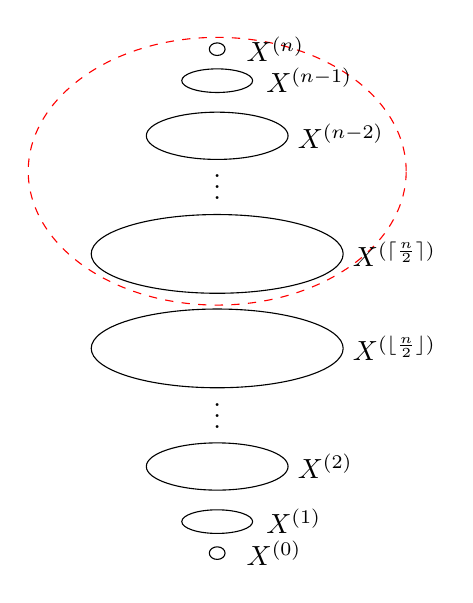
\begin{tikzpicture}
    \draw [red, dashed] (0,1.65) circle [x radius=2.4cm, y radius=1.7cm];
    \begin{scope}
      \draw (0,3.2) circle [x radius=1mm, y radius=0.8mm];
      \node [right] at (0.25, 3.2) {$X^{(n)}$};

      \draw (0,2.8) circle [x radius=4.5mm, y radius=1.5mm];
      \node [right] at (0.5, 2.8) {$X^{(n-1)}$};

      \draw (0,2.1) circle [x radius=9mm, y radius=3mm];
      \node [right] at (0.9, 2.1) {$X^{(n-2)}$};

      \node at (0,1.55) {$\vdots$};

      \draw (0,0.6) circle [x radius=16mm, y radius=5mm];
      \node [right] at (1.6, 0.6) {$X^{(\ceil{\frac{n}{2}})}$};

      \draw (0,-0.6) circle [x radius=16mm, y radius=5mm];
      \node [right] at (1.6, -0.6) {$X^{(\floor{\frac{n}{2}})}$};

      \node at (0,-1.35) {$\vdots$};

      \draw (0,-2.1) circle [x radius=9mm, y radius=3mm];
      \node [right] at (0.9, -2.1) {$X^{(2)}$};

      \draw (0,-2.8) circle [x radius=4.5mm, y radius=1.5mm];
      \node [right] at (0.5, -2.8) {$X^{(1)}$};

      \draw (0,-3.2) circle [x radius=1mm, y radius=0.8mm];
      \node [right] at (0.25, -3.2) {$X^{(0)}$};
    \end{scope}
  \end{tikzpicture}
\end{center}
What if we insist $A \subset X^{(r)}$?

If $r > \frac{n}{2}$, this is a silly question, as we can take $\A = X^{(r)}$.
If $r = \frac{n}{2}$, the maximum is $\frac{1}{2} \binom nr$ - just choose one of $A,A^c$ for each $A \in X^{(r)}$.
So assume $r < \frac{n}{2}$.

Taking
\begin{equation*}\mathcal{A} = \set{A \in X^{(r)} | 1 \in A}\end{equation*}
gives $|\A| = \binom{n-1}{r-1} = \frac{r}{n} \binom nr$.
Could also try, e.g.\
\begin{equation*}\mathcal{B} = \set{A \in X^{(r)} | |A \cap \{1,2,3\}| \geq 2}.\end{equation*}
Try both on $[8]^{(3)}$:
\begin{gather*}
  |\A| = \binom{7}{2} = 21 \\
  |\mathcal{B}| = 1 + \binom{3}{2} \binom{5}{1} = 16 < 21.
\end{gather*}
where the first term counts the number of $|A \cap \{1,2,3\}| = 3$, and the second term counts $|A \cap \{1,2,3\}| = 2$.

In fact, the size from $\A$ is optimal:
\begin{nthm}[Erd\H{o}s-Ko-Rado]\label{thm:ekr11}\index{Erd\H{o}s-Ko-Rado theorem}
  Let $r < \frac{n}{2}$, and let $\A \subset X^{(r)}$ be \hyperlink{def:inter}{intersecting}.
  Then $|\A| \leq \binom{n-1}{r-1}$.
\end{nthm}
\begin{proof}[Proof 1: `Bubble down with \nameref{thm:kk7}']
  For $A,B \in \A$, have $A \cap B \neq 0$, i.e.\ $A \nsubseteq B^c$.
  Writing $\bar{\A}$ for $\set{A^c | A \in \A} \subset X^{(n-r)}$, this says that $\partial^{n-2r} \bar{\A}$ is disjoint from $\A$.

  Suppose $|\A| > \binom{n-1}{r-1}$.
  Then $|\A^c| > \binom{n-1}{r-1} = \binom{n-1}{n-r}$, so by \nameref{thm:kk7} (as given in \cref{cor:9}), have $|\partial^{n-2r} \bar{\A}| \geq \binom{n-1}{r}$.
  But
  \begin{equation*}
    \binom{n-1}{r-1} + \binom{n-1}{r} = \binom{n}{r}
  \end{equation*}
  i.e.\
  \begin{equation*}
    |\partial^{n-2r} \bar{\A}| + |\A| > |X^{(r)}|.
  \end{equation*}
  a contradiction.
\end{proof}
\begin{remark}
  The numbers \emph{had} to work, as we get equality for $\A = \set{A \in X^{(r)} | 1 \in A}$.
\end{remark}
\begin{proof}[Proof 2]
  Consider a cyclic ordering of $[n]$, i.e.\ a bijection $C: [n] \to \mathbb{Z}_n$, e.g.
  \begin{center}
    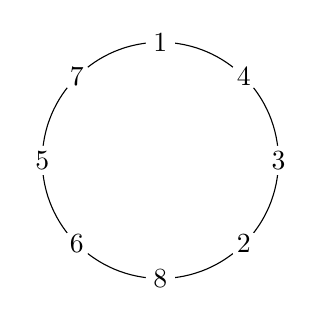
\begin{tikzpicture}[scale=1.5]
      \draw (0,0) circle [radius = 1cm];
      \begin{scope}[every node/.style={fill=white, circle, inner sep=0.3mm}]
      \node at (90:1) {1};
      \node at (45:1) {4};
      \node at (0:1) {3};
      \node at (-45:1) {2};
      \node at (-90:1) {8};
      \node at (-135:1) {6};
      \node at (180:1) {5};
      \node at (135:1) {7};
      \end{scope}
    \end{tikzpicture}
  \end{center}
  How many $A \in \A$ are intervals (sets of $r$ consecutive elements) in our ordering?
  Answer: $\leq r$. Indeed, suppose $c_1 \dots c_r \in \mathcal{A}$.
  Then, for each $1 \leq i \leq r-1$, at most one of the two intervals $\dots c_{i-1} c_i$ and $c_{i+1} c_{i+2} \dots$ can belong to $\A$.

  Also, a given $r$-set $A$ is an interval in exactly $n r! (n-r)!$ of the $n!$ cyclic orderings.
  Hence $|\A| n r! (n-r)! \leq n! r$, i.e.
  \begin{equation*}
    |\A| \leq \frac{(n-1)!}{(r-1)! (n-r)!} = \binom{n-1}{r-1}. \qedhere
  \end{equation*}
\end{proof}
\begin{remark}\leavevmode
  \begin{enumerate}
    \item Equivalently, we are double-counting the edges in the bipartite graph, vertex classes $\A$ and all cyclic orderings, in which $A$ is joined to $C$ if $A$ is an interval in $C$.
    \item This method is called \named{averaging}, or Katona's method.
  \end{enumerate}
\end{remark}
Equality in \nameref{thm:ekr11}? Can check equality holds $\iff \A = \set{A \in X^{(r)} | i \in A}$ for some $i$.
This follows (proof 1) from equality case of \nameref{thm:kk7}, or (proof 2) by considering changing the cyclic ordering bit by bit.
\clearpage
\section{Isoperimetric inequalities}
`How tightly can we pack a subset of given size in a space?'
\marginnote{\emph{Lecture 7}}[0cm]We are familiar with this kind of inequality in the continuous sense:
\begin{itemize}
  \item Among subsets of $\mathbb{R}^2$ of given area, the disc has smallest perimeter.
  \item Among subsets of $\mathbb{R}^3$ of given volume, the sphere has smallest surface area.
  \item Among subsets of $S^2$ of given area, the cap has smallest perimeter.
\end{itemize}

\begin{center}
  \begin{tikzpicture}[scale=1.5]
    \begin{scope}
      \draw [fill=bred!20] (0,0) circle [radius=1cm];
    \end{scope}
    \begin{scope}[xshift=3cm]
      \shade [ball color = bred!40, opacity = 0.7] (0,0) circle (1cm);
      \draw [very thin] (0,0) circle (1cm);
      \draw [very thin] (-1,0) arc (180:360:1 and 0.3);
      \draw [dashed, very thin] (1,0) arc (0:180:1 and 0.3);
    \end{scope}
    \begin{scope}[xshift=6cm]
      %\draw [dashed, very thin] (1,0) arc (0:180:1 and 0.3);
      %\draw [ultra thin] (0,0) circle (1cm);
      %\draw [ultra thin] (-1,0) arc (180:360:1 and 0.3);
      \shade [ball color = bred!40, opacity = 0.3] (0,0) circle (1cm);
    \begin{scope}
      \clip (0.33, 0.4) circle [x radius=0.32cm, y radius=0.28cm, rotate=125];
    \shade [ball color = bred!60, opacity = 0.4] (0,0) circle (1cm);
    \end{scope}
    \draw [ultra thin] (0.33, 0.4) circle [x radius=0.32cm, y radius=0.28cm, rotate=125];
    \end{scope}
  \end{tikzpicture}
\end{center}

\begin{defi}[Boundary]\hypertarget{def:boundary}
  For a set $A$ of vertices in a graph $G$, the \named{boundary} is
  \begin{equation*}
    b(A) = \set{x \in V(G) | x \notin A, xy \in E \text{ for some } y \in A}.
  \end{equation*}
\end{defi}
For example, in the picture, if $A = \{1,2,3\}$, then $b(A) = \{4,5\}$.
\begin{center}
  \begin{tikzpicture}
    \begin{scope}[every node/.style={draw=black, inner sep=1.5pt, circle}]
      \node[fill=bred, label=above:{$1$}] (1) at (0,1) {};
      \node[fill=bred, label=above:{$2$}] (2) at (1,1) {};
      \node[fill=bred, label=below:{$3$}] (3) at (0,0) {};
      \node[fill=bgreen, label=below:{$4$}] (4) at (1,0) {};
      \node[fill=bgreen, label=above:{$5$}] (5) at (2,1) {};
      \node[label=above:{$6$}] (6) at (3,1) {};
      \node[label=below:{$7$}] (7) at (2,0) {};
      \node[label=below:{$8$}] (8) at (3,0) {};
      \draw (2) -- (4) -- (3) -- (1) -- (2) -- (5) -- (6) -- (8) -- (7) -- (5);
  \end{scope}
  \end{tikzpicture}
\end{center}

\begin{defi}[Isoperimetric inequality]
An \named{isoperimetric inequality} on $G$ is an inequality of the form
\begin{equation*}
  |\hyperlink{def:boundary}{b(A)}| \geq f(|A|) \quad \forall \subseteq V(G).
\end{equation*}
\end{defi}

\begin{defi}[Neighbourhood]\hypertarget{def:neighbourhood}
Equivalently, minimise the \named{neighbourhood} of $A$:
\begin{equation*}
  N(A) = A \cap \hyperlink{def:boundary}{b(A)} = \set{x \in G | d(x,A) \leq 1}
\end{equation*}
where $d$ denotes the usual graph distance.
\end{defi}

A natural guess to minimise \hyperlink{def:neighbourhood}{neighbourhood} is often $B(x,r) = \set{y \in G | d(x,y) \leq r}$.
What happens in $Q_n$?
For example, try $|A|=4$ in $Q_3$:
\begin{center}
  \begin{tikzpicture}[scale=2]
    \node at (0.65,-0.3) {$|b(A)| = 3$};
    \node at (3.65,-0.3) {$|b(A)| = 4$};
    \begin{scope}[every node/.style={draw=black, inner sep=1.5pt, circle}]
      \node [fill=bred  ] (A) at (0,0) {};
      \node [fill=bred  ] (B) at (1,0) {};
      \node [fill=bgreen] (C) at (1,1) {};
      \node [fill=bred  ] (D) at (0,1) {};
      \node [fill=bred  ] (E) at (0.3,0.4) {};
      \node [fill=bgreen] (F) at (1.3,0.4) {};
      \node               (G) at (1.3,1.4) {};
      \node [fill=bgreen] (H) at (0.3,1.4) {};
      \draw (A) -- (B) -- (C) -- (D) -- (A);
      \draw (E) -- (F) -- (G) -- (H) -- (E);
      \draw (A) -- (E);
      \draw (B) -- (F);
      \draw (C) -- (G);
      \draw (D) -- (H);

      \begin{scope}[xshift=3cm]
        \node [fill=bred  ] (A) at (0,0) {};
        \node [fill=bred  ] (B) at (1,0) {};
        \node [fill=bgreen] (C) at (1,1) {};
        \node [fill=bgreen] (D) at (0,1) {};
        \node [fill=bred  ] (E) at (0.3,0.4) {};
        \node [fill=bred  ] (F) at (1.3,0.4) {};
        \node [fill=bgreen] (G) at (1.3,1.4) {};
        \node [fill=bgreen] (H) at (0.3,1.4) {};
        \draw (A) -- (B) -- (C) -- (D) -- (A);
        \draw (E) -- (F) -- (G) -- (H) -- (E);
        \draw (A) -- (E);
        \draw (B) -- (F);
        \draw (C) -- (G);
        \draw (D) -- (H);
      \end{scope}
  \end{scope}
  \end{tikzpicture}
\end{center}

Guess: `Balls are best', i.e.\
\begin{equation*}
  \text{if }|A| = |X^{(\leq r)}|,\text{ then }|\hyperlink{def:neighbourhood}{N(A)}| \geq |X^{(\leq r + 1)}|
\end{equation*}
\hypertarget{def:superrange}(where $X^{(\leq r)}$ is shorthand for $\hyperlink{def:superr}{X^{(0)}} \cup \dotsb \cup X^{(r)}$).

But what if $|A|$ is strictly between $\sum_{i=0}^r \binom{n}{i}$ and $\sum_{i=0}^{r+1} \binom{n}{i}$?
Guess: Take $A = X^{(\leq r)} \cup B$, for some $B \subset \hyperlink{def:superr}{X^{(r+1)}}$ (called a \hypertarget{def:hamming}`Hamming Ball'\index{Hamming ball}).
If we knew this, then
\begin{equation*}\hyperlink{def:neighbourhood}{N(A)} = X^{(\leq r+1)} \cup \hyperlink{def:upshad}{\partial^+} B,\end{equation*}
so by \nameref{thm:kk7} we'd take $B$ to be an initial segment of \hyperlink{def:lex}{lex}.

\begin{defi}[Simplicial order]\hypertarget{def:simplicial}
  Define the \named{simplicial order} on $Q_n$ by $x<y$ if either $|x| < |y|$ or $|x|=|y|$ and $x<y$ in \hyperlink{def:lex}{lex}.
\end{defi}
The slogan for the \hyperlink{def:simplicial}{simplicial order} is `Go up in levels, and use \hyperlink{def:lex}{lex} inside a level.'
\begin{aim}
Initial segments of \hyperlink{def:simplicial}{simplicial} order are best for minimising $\hyperlink{def:neighbourhood}{N(A)}$.
\end{aim}

\begin{defi}[Sections]\hypertarget{def:section}
  Given $A \subset \hyperlink{def:qn}{Q_n}$ and $1 \leq i \leq n$, the \index{section}\textbf{$i$-sections} are the \hyperlink{def:ss}{set systems} $A_+^{(i)}, A_-^{(i)} \subset \mathcal{P}(X-i)$ given by
  \begin{gather*}
    A_-^{(i)} = \set{ x \in A | i \notin x} \subset \mathcal{P}(X-\{i\}) \\
    A_+^{(i)} = \set{ x - \{i\} | x \in A, i \in x} \subset \mathcal{P}(X-\{i\}).
  \end{gather*}
  Note $\mathcal{P}(X-\{i\})$ is \hyperlink{def:iso}{isomorphic} to $\hyperlink{def:qn}{Q_{n-1}}$.
  \begin{center}
    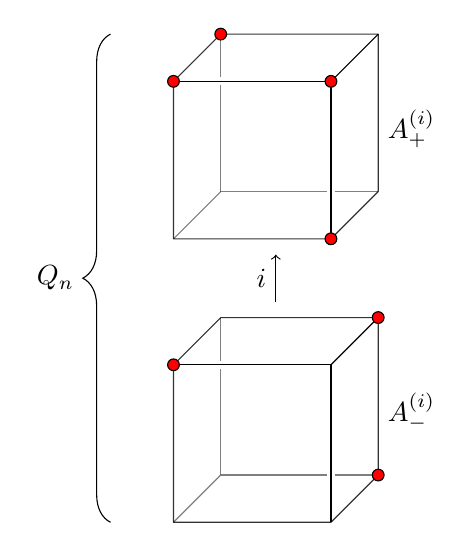
\begin{tikzpicture}[scale=2]
      \begin{scope}[every node/.style={inner sep=0, minimum size=0, outer sep=0}, mymark/.style={inner sep=1.5pt, draw=black, fill=red, circle}, over/.style={white, line width=1.2pt, double distance=0.4pt, shorten < = 1pt}]
        \begin{scope}
          \node (A) at (0,0) {};
          \node (B) at (1,0) {};
          \node (C) at (1,1) {};
          \node (D) at (0,1) {};
          \node (E) at (0.3,0.3) {};
          \node (F) at (1.3,0.3) {};
          \node (G) at (1.3,1.3) {};
          \node (H) at (0.3,1.3) {};
          \foreach \x in {A,F,H} {\draw [opacity=0.5] (E) -- (\x);};
          \foreach \x in {B,D,G} {\draw [over] (C) -- (\x); \draw (C) -- (\x);};
          \draw [line cap=round, opacity=0.8] (A) -- (B) -- (F) -- (G) -- (H) -- (D) -- (A);
          \foreach \x in {B,C,D,H} {\node [mymark] at (\x) {};}
        \end{scope}
        \begin{scope}[yshift=-1.8cm]
          \node (A) at (0,0) {};
          \node (B) at (1,0) {};
          \node (C) at (1,1) {};
          \node (D) at (0,1) {};
          \node (E) at (0.3,0.3) {};
          \node (F) at (1.3,0.3) {};
          \node (G) at (1.3,1.3) {};
          \node (H) at (0.3,1.3) {};
          \foreach \x in {A,F,H} {\draw [opacity=0.5] (E) -- (\x);};
          \foreach \x in {B,D,G} {\draw [over] (C) -- (\x); \draw (C) -- (\x);};
          \draw [line cap=round, opacity=0.8] (A) -- (B) -- (F) -- (G) -- (H) -- (D) -- (A);
          \foreach \x in {D,F,G} {\node [mymark] at (\x) {};}
        \end{scope}
      \end{scope}
      \draw [->] (0.65, -0.4) -- (0.65, -0.1) node [left, midway] {$i$};
      \node [right] at (1.3, 0.7) {$A_+^{(i)}$};
      \node [right] at (1.3, -1.1) {$A_-^{(i)}$};
      \draw [decorate,decoration={brace,amplitude=10pt}, xshift=-0.4cm] (0,-1.8) -- (0,1.3) node [black,midway,xshift=-0.7cm] {$Q_n$};
    \end{tikzpicture}
  \end{center}
\end{defi}
\begin{defi}[Compression]\hypertarget{def:icomp}
  Define the \textbf{$i$-compression} $C_i(A)$ of $A$ by giving its \hyperlink{def:section}{$i$-sections}.
  \begin{itemize}
    \item $C_i(A)_+^{i}$ is the initial segment of $Q_{n-1}$ of size $|A^{(i)}_+|$
    \item $C_i(A)_-^{i}$ is the initial segment of $Q_{n-1}$ of size $|A^{(i)}_-|$
  \end{itemize}
\end{defi}
\begin{center}
  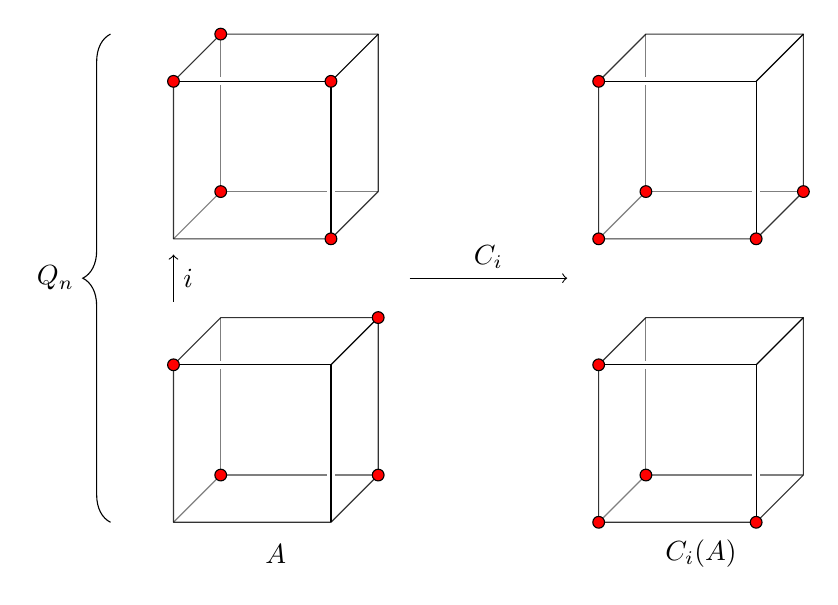
\begin{tikzpicture}[scale=2]
    \begin{scope}[every node/.style={inner sep=0, minimum size=0, outer sep=0}, mymark/.style={inner sep=1.5pt, draw=black, fill=red, circle}, over/.style={white, line width=1.2pt, double distance=0.4pt, shorten < = 1pt}]
      \begin{scope}
        \node (A) at (0,0) {};
        \node (B) at (1,0) {};
        \node (C) at (1,1) {};
        \node (D) at (0,1) {};
        \node (E) at (0.3,0.3) {};
        \node (F) at (1.3,0.3) {};
        \node (G) at (1.3,1.3) {};
        \node (H) at (0.3,1.3) {};
        \foreach \x in {A,F,H} {\draw [opacity=0.5] (E) -- (\x);};
        \foreach \x in {B,D,G} {\draw [over] (C) -- (\x); \draw (C) -- (\x);};
        \draw [line cap=round, opacity=0.8] (A) -- (B) -- (F) -- (G) -- (H) -- (D) -- (A);
        \foreach \x in {B,C,D,E,H} {\node [mymark] at (\x) {};}
      \end{scope}
      \begin{scope}[yshift=-1.8cm]
        \node (A) at (0,0) {};
        \node (B) at (1,0) {};
        \node (C) at (1,1) {};
        \node (D) at (0,1) {};
        \node (E) at (0.3,0.3) {};
        \node (F) at (1.3,0.3) {};
        \node (G) at (1.3,1.3) {};
        \node (H) at (0.3,1.3) {};
        \foreach \x in {A,F,H} {\draw [opacity=0.5] (E) -- (\x);};
        \foreach \x in {B,D,G} {\draw [over] (C) -- (\x); \draw (C) -- (\x);};
        \draw [line cap=round, opacity=0.8] (A) -- (B) -- (F) -- (G) -- (H) -- (D) -- (A);
        \foreach \x in {D,E,F,G} {\node [mymark] at (\x) {};}
      \end{scope}
      \begin{scope}[xshift=2.7cm]
        \node (A) at (0,0) {};
        \node (B) at (1,0) {};
        \node (C) at (1,1) {};
        \node (D) at (0,1) {};
        \node (E) at (0.3,0.3) {};
        \node (F) at (1.3,0.3) {};
        \node (G) at (1.3,1.3) {};
        \node (H) at (0.3,1.3) {};
        \foreach \x in {A,F,H} {\draw [opacity=0.5] (E) -- (\x);};
        \foreach \x in {B,D,G} {\draw [over] (C) -- (\x); \draw (C) -- (\x);};
        \draw [line cap=round, opacity=0.8] (A) -- (B) -- (F) -- (G) -- (H) -- (D) -- (A);
        \foreach \x in {A,B,D,E,F} {\node [mymark] at (\x) {};}
      \end{scope}
      \begin{scope}[xshift=2.7cm, yshift=-1.8cm]
        \node (A) at (0,0) {};
        \node (B) at (1,0) {};
        \node (C) at (1,1) {};
        \node (D) at (0,1) {};
        \node (E) at (0.3,0.3) {};
        \node (F) at (1.3,0.3) {};
        \node (G) at (1.3,1.3) {};
        \node (H) at (0.3,1.3) {};
        \foreach \x in {A,F,H} {\draw [opacity=0.5] (E) -- (\x);};
        \foreach \x in {B,D,G} {\draw [over] (C) -- (\x); \draw (C) -- (\x);};
        \draw [line cap=round, opacity=0.8] (A) -- (B) -- (F) -- (G) -- (H) -- (D) -- (A);
        \foreach \x in {A,B,D,E} {\node [mymark] at (\x) {};}
      \end{scope}
    \end{scope}
    \draw [->] (0, -0.4) -- (0, -0.1) node [right, midway] {$i$};
    \node at (0.65,-2) {$A$};
    \node at (3.35,-2) {$C_i(A)$};
    \draw [->] (1.5, -0.25) -- (2.5, -0.25) node [above, midway] {$C_i$};
    \draw [decorate,decoration={brace,amplitude=10pt}, xshift=-0.4cm] (0,-1.8) -- (0,1.3) node [midway,xshift=-0.7cm] {$Q_n$};
  \end{tikzpicture}
\end{center}
Certainly $|\hyperlink{def:icomp}{C_i(A)}| = |A|$.
Also, $C_i(A)$ `looks more like' an initial segment of \hyperlink{def:simplicial}{simplicial} than $A$ did.

Say $A$ is \textbf{$i$-compressed} if $\hyperlink{def:icomp}{C_i(A)} = A$.

\begin{nthm}[Harper's theorem]\label{thm:harper1}
  Let $A \subset \hyperlink{def:qn}{Q_n}$, and let $C$ be the initial segment of \hyperlink{def:simplicial}{simplicial} order with $|C| = |A|$.
  Then $|\hyperlink{def:neighbourhood}{N(A)}| \geq |N(C)|$.
  In particular, if
  \begin{equation*}|A| \geq \sum_{i=0}^r \binom{n}{i}\end{equation*}
  then
  \begin{equation*}|N(A)| \geq \sum_{i=0}^{r+1} \binom{n}{i}.\end{equation*}
\end{nthm}
\begin{remark}\leavevmode
  \begin{enumerate}[label=\arabic*.]
    \item If we know $A$ is a \hyperlink{def:hamming}{Hamming ball}, then done by \nameref{thm:kk7}.
    \item \nameref{thm:harper1} $\Rightarrow$ \nameref{thm:kk7}: Given $B \subset X^{(r)}$, apply \nameref{thm:harper1} to $A = B \cup X^{(\leq r-1)}$
  \end{enumerate}
\end{remark}
\begin{proof}
  Induction on $n$. $n=1$ works.
  Given $A \subset Q_n$ for $n > 1$, fix $1 \leq i \leq n$.

  \textbf{Claim:} $|N(\hyperlink{def:icomp}{C_i(A)})| \leq |\hyperlink{def:neighbourhood}{N(A)}|$.

  \textbf{Proof of claim:} Write $B = C_i(A)$.
  We have
  \begin{align*}
    |N(A)| &= |A_+ \cup N(A_-)| + |A_- \cup N(A_+)| \\
    |N(B)| &= |B_+ \cup N(B_-)| + |B_- \cup N(B_+)|
  \end{align*}
  where the first term is `downstairs', and the second term is `upstairs'.
  Now, $|B_+| = |A_+|$ and $|N(B_-)| \leq |N(A_-)|$ by induction.

  But $N(B_-)$ is an initial segment of \hyperlink{def:simplicial}{simplicial} on $Q_{n-1}$ as is $B_+$.
  So $N(B_-)$ and $B_+$ are nested (in some direction).
  Hence
  \begin{align*}
    |B_+ \cup N(B_-)| &\leq |A_+ \cup N(A_-)| \\
    \shortintertext{and similarly}
    |B_- \cup N(B_+)| &\leq |A_- \cup N(A_+)|
  \end{align*}
  Thus $|N(B)| \leq |N(A)|$. $\blacksquare$

  \marginnote{\emph{Lecture 8}}[0cm]Among all $B \subset Q_n$ with $|B| = |A|$ and $|N(B)| \leq |N(A)|$, choose one with
  \begin{equation*}
    \sum_{x \in B} f(x)
  \end{equation*}
  minimal, where $f(x)=$ the position of $x$ in the \hyperlink{def:simplicial}{simplicial order} on $Q_n$.
  Then $B$ is $i$-compressed $\forall i$.
  Must such a $B$ be an initial segment of simplicial?
  Unfortunately, no - e.g.\ $B = \{\emptyset,1,2,12\} \subset Q_3$.

  However,
  \begin{nlemma}\label{lem:2.2}
    Let $B \subset Q_n$ be $i$-compressed $\forall i$ but not an initial segment of simplicial order.
    Then if $n$ is odd, say $n = 2k+1$, we have
    \begin{align*}
      B &= X^{(\leq k)} - \{\text{last $k$-set}\} \cup {\{\text{first $k+1$-set}\}}\\ % mark the last kset as (k+2),...,(2k+1) and the first as 1,2,...,k,(k+1)
        &= X^{(\leq k)} - \{(k+2) \dotsc (2k+1)\} \cup \{12\dotsc k(k+1)\}
    \end{align*}
    while if $n$ is even, say $n = 2k$, we have
    \begin{align*}
      B &= X^{(\leq k-1)} \cup \set{x \in X^{(k)} | 1 \in x} - \{\text{last $k$-set with 1}\} \cup \{\text{first $k$-set without $1$}\}\\ % mark the last kset as 1(k+2),...,(2k) and the first as 2,3,4,...,k,(k+1)
        &= X^{(\leq k-1)} \cup \set{x \in X^{(k)} | 1 \in x} - \{1(k+2)\dotsc(2k)\} \cup \{234\dotsc k(k+1)\}
    \end{align*}
  \end{nlemma}

  \begin{center}
    \begin{tikzpicture}
      \begin{scope}
        \node at (-2, 3) {$n=2k$};

        \draw (0,3.2) circle [x radius=1mm, y radius=1mm];
        \draw (0,2.7) circle [x radius=4.5mm, y radius=2mm];
        \draw (0,1.9) circle [x radius=9mm, y radius=4mm];

        \node at (0,1.25) {$\vdots$};

        \begin{scope}
          \clip (0,0) circle [x radius=16mm, y radius=8mm];
          \fill [bred!40] (-1.6,-0.8) -- (0.2,-0.8) arc (0:90:2mm) -- (0,0.6) arc (-90:-180:2mm) -- (-1.6,0.8) -- cycle;
          \draw [very thin] (0,0.8) -- (0,-0.8);
        \end{scope}
        \draw (0,0) circle [x radius=16mm, y radius=8mm];
        \node [right] at (1.6, 0) {$X^{(k)}$};
        \node at (-1.3,0.9) {$1 \in$};
        \node at (1.3,0.9) {$1 \notin$};

        \node at (0,-1.05) {$\vdots$};

        \draw [fill=bred!40] (0,-1.9) circle [x radius=9mm, y radius=4mm];
        \draw [fill=bred!40] (0,-2.7) circle [x radius=4.5mm, y radius=2mm];
        \draw [fill=bred!40] (0,-3.2) circle [x radius=1mm, y radius=1mm];
      \end{scope}

      \begin{scope}[xshift=6cm]
        \node at (-2, 3) {$n=2k+1$};

        \draw (0,3.2) circle [x radius=1mm, y radius=0.8mm];
        \draw (0,2.8) circle [x radius=4.5mm, y radius=1.5mm];
        \draw (0,2.1) circle [x radius=9mm, y radius=3mm];

        \node at (0,1.55) {$\vdots$};

        \begin{scope}
          \clip (0,0.6) circle [x radius=16mm, y radius=5mm];
          \fill [bred!40] (-1.9,0.6) circle [radius=5mm];
        \end{scope}
        \draw (0,0.6) circle [x radius=16mm, y radius=5mm];
        \node [right] at (1.6, 0.6) {$X^{(k+1)}$};

        \begin{scope}
          \clip (0,-0.6) circle [x radius=16mm, y radius=5mm];
          \fill [bred!40] (1.9,-0.6) circle [radius=5mm] (-1.6,-1.1) rectangle (1.6,-0.1);
        \end{scope}
        \draw (0,-0.6) circle [x radius=16mm, y radius=5mm];
        \node [right] at (1.6, -0.6) {$X^{(k)}$};

        \node at (0,-1.35) {$\vdots$};

        \draw [fill=bred!40] (0,-2.1) circle [x radius=9mm, y radius=3mm];
        \draw [fill=bred!40] (0,-2.8) circle [x radius=4.5mm, y radius=1.5mm];
        \draw [fill=bred!40] (0,-3.2) circle [x radius=1mm, y radius=0.8mm];
      \end{scope}
    \end{tikzpicture}
  \end{center}
  Once we have proved this, we are done, as in each case $|N(B)| \geq |N(C)|$.
  \begin{proof}
    We have $x \notin B, y \in B$ for some $x,y$ with $x<y$ in simplicial.
    We cannot have $i \in x, i \in y$ (as $B$ is $i$-compressed), and cannot have $i \notin x, i \notin y$ (as $B$ is $i$-compressed).

    So, for each $i$, $i$ belongs to exactly one of $x,y$.
    Thus $y = x^c$.

    Hence for each $y \in B$, at most one $x < y$ has $x \notin B$ (namely $y^c$) and for each $x \notin B$, at most $y > x$ has $y \in B$ (namely $x^c$).

    Hence $B = \set{z | z \leq y} - \{x\}$ where $x$ is the immediate predecessor of $y$ and $x = y^c$.
    But then $x=$ last $k$-set (if $n=2k+1$) or the last $k$-set containing $1$ (if $n = 2k$)
    by definition of simplicial ordering.
  \end{proof}
\end{proof}

\begin{remark}\leavevmode
  \begin{enumerate}[label=\arabic*.]
    \item Can also prove \nameref{thm:harper1} by \hyperlink{def:uvcomp}{$UV$-compressions}.
    \item Can also use these `codimension 1' compressions to prove \nameref{thm:kk7}.
  \end{enumerate}
\end{remark}
\begin{defi}[Neighbourhood]
  \hypertarget{def:tneighbourhood}For $A \subset Q_i$, the \textbf{$t$-neighbourhood} of $A$ is
  \begin{equation*}
    A_{(t)} \coloneqq N^t(A) = \set{x \in Q_n | d(x,A) \leq t}.
  \end{equation*}
\end{defi}
\begin{ncor}\label{cor:2.3}
  Let $A \subset \hyperlink{def:qn}{Q_n}$ with $|A| = |\hyperlink{def:superrange}{X^{(\leq r)}}|$. Then, for $1 \leq t \leq n-r$, have
  \begin{equation*}
    |\hyperlink{def:tneighbourhood}{A_{(t)}}| \geq |X^{(\leq r + t)}|
  \end{equation*}
\end{ncor}
\begin{proof}
  \nameref{thm:harper1} and induction.
\end{proof}
To get a feel for what \cref{cor:2.3} is saying, we'll need some estimates for things like $\sum_{i=0}^r \binom{n}{i}$.
\begin{nprop}\label{prop:2.4}
  Let $0 \leq \epsilon < \frac{1}{4}$, then
  \begin{equation*}
    \sum_{i=0}^{\floor{(\frac{1}{2} - \epsilon) n}} \binom{n}{i} < \frac{1}{\epsilon} e^{(-\epsilon^2 \frac{n}{2})} 2^n
  \end{equation*}
  (an exponentially small fraction of $2^n$ for $\epsilon$ fixed).
\end{nprop}
Roughly we are going around $\epsilon \sqrt{n}$ standard deviations from the mean.

\begin{proof}
  For $i \leq (\frac{1}{2} - \epsilon) n:$
  \begin{equation*}
    \frac{\binom{n}{i-1}}{\binom{n}{i}} = \frac{i}{n-i+1} \leq \frac{\frac{1}{2} - \epsilon}{\frac{1}{2} + \epsilon} = 1 - \frac{2\epsilon}{\frac{1}{2} + \epsilon} \leq 1 - 2\epsilon.
  \end{equation*}
  Hence
  \begin{equation*}
    \sum_{i=0}^{\floor{(\frac{1}{2}-\epsilon) n}} \binom{n}{i} \leq \frac{1}{2\epsilon} \binom{n}{\floor{(\frac{1}{2} - \epsilon) n}}
  \end{equation*}
  as a geometric progression.
  Similarly, replacing $\epsilon$ with $\frac \epsilon 2$,
  \begin{align*}
    \binom{n}{\floor{(\frac{1}{2} - \epsilon)n}} &\leq (1-\epsilon)^{\epsilon \frac{n}{2} - 1} \binom{n}{\floor{(\frac{1}{2} - \frac{\epsilon}{2}) n}} \\
                                                 &\leq 2(1-\epsilon)^{\frac \epsilon 2} 2^n \\
                                                 &\leq 2 e^{-\epsilon \cdot \epsilon \frac n2} 2^n,
  \end{align*}
  using $e^{-x} \geq 1-x$ in the final step.
  Thus
  \begin{equation*}
    \sum_{i=0}^{\floor{(\frac{1}{2} - \epsilon) n}} \binom{n}{i}\leq \frac{1}{2\epsilon} 2 e^{-\epsilon^2 \frac{n}{2}} \cdot 2^n. \qedhere
  \end{equation*}
\end{proof}

\begin{nthm}\label{thm:2.5}
  \marginnote{\emph{Lecture 9}}[0cm]
  Let $A \subset Q_n$ with $\frac{|A|}{2^n} \geq \frac{1}{2}$, and $0 < \epsilon < \frac{1}{4}$.
  Then
  \begin{equation*}
    \frac{|A_{(\epsilon n)|}}{2^n} \geq 1 - \frac{2}{\epsilon} e^{-\epsilon^2 \frac{n}{2}}.
  \end{equation*}
  `$\frac{1}{2}$-sized sets have exponentially large $\epsilon n$-neighbourhoods'
\end{nthm}
\begin{proof}
  Enough to show that if $\epsilon n$ an integer, then
  \begin{equation*}
    \frac{|A_{(\epsilon n)}|}{2^n} \geq 1 - \frac{1}{\epsilon} e^{-\epsilon^2 \frac{n}{2}}.
  \end{equation*}
  We have
  \begin{equation*}
    |A| \geq \sum_{i=0}^{\ceil{\frac{n}{2} - 1}} \binom{n}{i}
  \end{equation*}
  So by \nameref{thm:harper1}, we have
  \begin{equation*}
    |A_{(\epsilon n)}| \geq \sum_{i=0}^{\ceil{n(\frac{1}{2} + \epsilon) - 1}} \binom{n}{i}
  \end{equation*}
  i.e.,
  \begin{equation*}
    |{A_{(\epsilon n)}}^c| \leq \sum_{i=\ceil{n (\frac{1}{2} + \epsilon)}}^n \binom{n}{i} = \sum_{i=0}^{\floor{n(\frac{1}{2}- \epsilon)}} \binom{n}{i} \leq \frac{1}{\epsilon} e^{-\epsilon^2 \frac{n}{2}} \cdot 2^n. \qedhere
  \end{equation*}
\end{proof}
\subsection{Concentration of measure}
\begin{defi}[Lipschitz]\hypertarget{def:lips}
Say $f: Q_n \to \mathbb{R}$ is \named{Lipschitz} if $|f(x) - f(y)| \leq 1$ for all $x,y \in \hyperlink{def:qn}{Q_n}$ adjacent.
\end{defi}

\begin{defi}[Median]\hypertarget{def:median}
Say $M \in \mathbb{R}$ is a \named{median} or \textbf{L\'evy mean} of $f$ if
\begin{equation*}
  |\set{x | f(x) \leq M}|,\ |\set{x | f(x) \geq M}| \geq \frac{1}{2} \cdot 2^n.
\end{equation*}
\end{defi}
Now ready to show `every well-behaved function on \hyperlink{def:qn}{$Q_n$} is roughly constant nearly everywhere'.

\begin{nthm}\label{thm:2.6}
  Let $f: \hyperlink{def:qn}{Q_n} \to \mathbb{R}$ be \hyperlink{def:lips}{Lipschitz} with \hyperlink{def:median}{median} $M$, and $0 < \epsilon < \frac{1}{4}$.
  Then
  \begin{equation*}
    \frac{\left\lvert\Set{x | \lvert f(x) - M \rvert \leq \epsilon n}\right\rvert}{2} \geq 1 - \frac{4}{\epsilon} e^{-\epsilon^2 \frac{n}{2}}.
  \end{equation*}
\end{nthm}
\begin{proof}
  Let $A = \set{x | f(x) \leq M}$.
  Then $\frac{|A|}{2^n} \geq \frac{1}{2}$,
  so
  \begin{equation*}
    \frac{|A_{\epsilon n}|}{2^n} \geq 1 - \frac{2}{\epsilon} e^{-\epsilon^2 \frac{n}{2}}.
  \end{equation*}
  But $x \in A_{(\epsilon n)} \implies f(x) \leq M + \epsilon n$ (as $f$ is \hyperlink{def:lips}{Lipschitz}), so
  \begin{equation*}
    \frac{|\set{x | f(x) \leq M + \epsilon n}|}{2^n} \geq 1 - \frac{2}{\epsilon} e^{-\epsilon^2 \frac{n}{2}}.
  \end{equation*}
  Similarly,
  \begin{equation*}
    \frac{|\set{x | f(x) \leq M - \epsilon n}|}{2^n} \geq 1 - \frac{2}{\epsilon} e^{-\epsilon^2 \frac{n}{2}}
  \end{equation*}
  and intersect these.
\end{proof}

\begin{remark}
  This is the `\named{concentration of measure} phenomenon'.
\end{remark}
Let $G$ be a graph of diameter $D$ (recall the diameter is $\max\set{d(x,y) | x, y \in G}$).
Let
\begin{equation*}
  \alpha(G,\epsilon) = \max\Set{1 - \frac{\left\lvert \hyperlink{def:tneighbourhood}{A_{(\epsilon D)}}\right\rvert}{\left\lvert G \right\rvert} | A \subset G, \frac{|A|}{|G|} \geq \frac{1}{2}}.
\end{equation*}
So $\alpha(G,\epsilon)$ \emph{small} says `$\frac{1}{2}$-sized sets have big \hyperlink{def:tneighbourhood}{$\epsilon D$-neighbourhoods}.'

\begin{defi}[L\'evy family]\hypertarget{def:levyfam}
Say a sequence of graphs $G_1, G_2, \dotsc$ is a \named{L\'evy family} if $\alpha(G_n, \epsilon) \to 0$ as $n \to \infty$ (for each fixed $\epsilon$).
\end{defi}

Thus \cref{thm:2.5} says $Q_1, Q_2, Q_3, \dotsc$ forms a \hyperlink{def:levyfam}{L\'evy family} and even a \textbf{normal} L\'evy family, meaning $\alpha(G_n, \epsilon)$ exponentially small in $n$ (for each fixed $\epsilon$), so have concentration of measure as in (\cref{thm:2.6}) for any \hyperlink{def:levyfam}{L\'evy family}.

Many natural families of graphs form \hyperlink{def:levyfam}{L\'evy families}, e.g.\ symmetric group $S_n$ - made into a graph by joining $x,y$ if $x y^{-1}$ is a transposition.

Similarly, we can define $\alpha(X, \epsilon)$ for $X$ any metric measure space (of finite diameter and finite measure) - so again have concentration of measure for any \hyperlink{def:levyfam}{L\'evy family}.
\begin{eg}
  Take the sphere $S^n \subset \mathbb{R}^{n+1}$.
  \begin{center}
    \begin{tikzpicture}
      \node [left] at (-1.2,0) {$S^2 \subseteq \mathbb{R}^3$};
        \draw [dashed, very thin] (1,0) arc (0:180:1 and 0.3);
        \shade [ball color = bred!40, opacity = 0.5] (0,0) circle (1cm);
        \draw [very thin] (0,0) circle (1cm);
        \draw [very thin] (-1,0) arc (180:360:1 and 0.3);
    \end{tikzpicture}
  \end{center}
  To show `$\frac{1}{2}$-sized sets have big $\epsilon$-neighbourhoods', we need two ingredients:
  \begin{enumerate}[label=\arabic*)]
    \item An isoperimetric inequality: if $A \subset S^n$ and $C \subset S^n$ is the circular cap with $|C| = |A|$, then $|A_{(\epsilon)}| \geq |C_{(\epsilon)}|$.
      \begin{center}
        \begin{tikzpicture}[scale=2]
          \draw [dashed, very thin] (1,0) arc (0:180:1 and 0.3);
          \shade [ball color = bred!40, opacity = 0.5] (0,0) circle (1cm);
          \draw [very thin] (0,0) circle (1cm);
          \draw [very thin] (-1,0) arc (180:360:1 and 0.3);
          \begin{scope}[every path/.style={fill=white, fill opacity=0.5, very thin}]
            \draw (0.4, 0.4) circle [x radius=0.25cm, y radius=0.22cm, rotate=120];
            \draw [decorate, decoration={random steps, segment length=1.8pt, amplitude=1.2pt}] (-0.3, 0.2) circle [x radius=0.25cm, y radius=0.2cm, rotate=-10];
          \end{scope}
          \node at (-0.1,-0.1) {$A$};
          \node at (0.4,0) {$C$};
        \end{tikzpicture}
      \end{center}

  Compression is `stamp on your set', i.e.\ we always move a point above the equator to corresponding point below the equator, called 2-point symmetrisation.
      \begin{center}
        \begin{tikzpicture}[scale=1.5]
          \draw (0.3,0.5) -- (0.3,-0.5);
          \draw [dashed, very thin] (1,0) arc (0:180:1 and 0.3);
          \shade [ball color = bred!40, opacity = 0.5] (0,0) circle (1cm);
          \draw [very thin] (0,0) circle (1cm);
          \draw [very thin] (-1,0) arc (180:360:1 and 0.3);
          \node [circle, fill, inner sep=0.3mm] at (0.3,0.5) {};
          \node [circle, fill, inner sep=0.3mm] at (0.3,-0.5) {};
        \end{tikzpicture}
      \end{center}

    \item An estimate: Let $C$ be the circular cap with $|C| = \frac{1}{2}$, i.e.\ angle = $\frac{\pi}{2}$.
      \begin{center}
        \begin{tikzpicture}[scale=1.5]
            %\draw [very thin] (-0.979,0.2) arc (180:360:0.979 and 0.27);
            \draw [very thin] (-1,0) arc (180:360:1 and 0.3);
            %\draw [very thin] (0,0) circle (1cm);
          \begin{scope}
            \clip (-0.98,0.2) arc (180:360:0.98 and 0.27) -- (0,0.47) -- (-0.98,0.2);
            \clip (1,0) arc (0:180:1 and 0.3) -- (0,-0.3) -- (1,0);
            \begin{scope}[transform canvas={rotate=180}]
              \shade [ball color = red!60!black, opacity = 0.2] (0,0) circle (1cm);
            \end{scope}
          \end{scope}
          \begin{scope}
            \path [clip] (0,0.2) ellipse (0.98 and 0.27);
            \path [clip] (1,0) arc (0:180:1 and 0.3) -- (-1,0.47) -- (1,0.47) -- (1,0);
            \begin{scope}[transform canvas={rotate=180}]
              \shade [ball color = green!60!black, opacity = 0.2] (0,0) circle (1cm);
            \end{scope}
          \end{scope}
          \begin{scope}
            \clip (-0.98,0.2) arc (180:360:0.98 and 0.27) -- (1,0.2) -- (1,0) arc (360:180:1 and 0.3) -- (-1,0.2) -- (-0.98,0.2);
            \shade [ball color = bgreen!40, opacity = 0.5] (0,0) circle (1cm);
          \end{scope}
          \begin{scope}
            \path [clip] (-1,0) arc (180:360:1 and 0.3) -- (1,-1) -- (-1,-1) -- (-1,0);
            \shade [ball color = bred!40, opacity = 0.5] (0,0) circle (1cm);
          \end{scope}
        \end{tikzpicture}
      \end{center}
      Then $C_{(\epsilon)}$ is the circular cap of angle $\frac{\pi}{2} + \epsilon$. But the remaining volume is proportional to $\int_\epsilon^{\frac{\pi}{2}} (\cos \theta)^n \, d\theta$, which $\to 0$ (exponentially fast) as $n \to \infty$.
      %\begin{center}
      %  \begin{tikzpicture}[scale=2]
      %    \draw (0,1) to[out=-85, in=95] (0.02,0.5) to[out=-88] (0.1,0.01) to (1,0);
      %  \end{tikzpicture}
      %\end{center}
  \end{enumerate}
\end{eg}
We\marginnote{\emph{Lecture 10}} deduced concentration of measure from isoperimetric inequalities. Conversely,

\begin{nprop}\label{prop:2.7}
  Let $G$ be a graph such that for any \hyperlink{def:lips}{Lipschitz} function $G \to \mathbb{R}$ with median $M$, we have
  \begin{equation*}
    \frac{|\set{x \in G | |f(x) - M| \leq t}|}{|G|} \geq 1-\alpha
  \end{equation*}
  for some given $t,\alpha$.
  Then for $A \subset G$ with $\frac{|A|}{|G|} \geq \frac{1}{2}$, we have $\frac{|\hyperlink{def:tneighbourhood}{A_{(t)}}|}{|G|} \geq 1 - \alpha$.
\end{nprop}
\begin{proof}
  The function $f(x) = d(x,A)$ is Lipschitz and has $0$ as a median (as $|A| \geq \frac{1}{2} |G|$).
\end{proof}
\subsection{Edge-isoperimetric inequalities}
\begin{defi}[Edge boundary]\hypertarget{def:ebound}
For $A \subset G$ ($G$ a graph), the \textbf{edge-boundary} of $A$ is $\partial A = \set{xy \in E(G) | x \in A, y \notin A}$.
\end{defi}
\begin{center}
  \begin{tikzpicture}[scale=1.5]
    \begin{scope}[every node/.style={draw, circle, inner sep=1.5pt}]
      \node [label=below:$3$, fill=bred] (3) at (0  ,0) {};
      \node [label=below:$4$, fill=bred] (4) at (1  ,0) {};
      \node [label=above:$2$] (2) at (1  ,1) {};
      \node [label=above:$1$, fill=bred] (1) at (0  ,1) {};
      \node [label=above:$5$] (5) at (2.3,1) {};
      \node [label=below:$6$] (6) at (1.8,0) {};
      \node [label=below:$7$] (7) at (2.8,0) {};
      \draw [ultra thick, bgreen] (1) -- (2) -- (4);
      \draw (2) -- (4) -- (3) -- (1) -- (2) -- (5) -- (6) -- (7) -- (5);
      \draw (1) -- (4);
    \end{scope}
    \node at (1.4, -0.5) {$|{\color{bgreen}\partial A}| = 2$};
  \end{tikzpicture}
\end{center}
In $\hyperlink{def:qn}{Q_n}$ how should we choose $A$ (with $|A|$ given) to minimise $|\hyperlink{def:ebound}{\partial A}|$?

Take for example $|A|=4$ in $Q_3$:
\begin{center}
  \begin{tikzpicture}[scale=2]
    \begin{scope}[every node/.style={inner sep=0, minimum size=0, outer sep=0}, mymark/.style={inner sep=1.5pt, draw=black, fill=red, circle}, over/.style={white, line width=1.2pt, double distance=0.4pt, shorten < = 1pt}]
      \begin{scope}
        \node (A) at (0,0) {};
        \node (B) at (1,0) {};
        \node (C) at (1,1) {};
        \node (D) at (0,1) {};
        \node (E) at (0.3,0.3) {};
        \node (F) at (1.3,0.3) {};
        \node (G) at (1.3,1.3) {};
        \node (H) at (0.3,1.3) {};
        \foreach \x in {A,F,H} {\draw [opacity=0.5] (E) -- (\x);};
        \draw [line cap=round, ultra thick, bgreen, opacity=0.5] (E) -- (F);
        \draw [line cap=round, ultra thick, bgreen, opacity=0.5] (E) -- (H);
        \foreach \x in {B,D,G} {\draw [over] (C) -- (\x); \draw (C) -- (\x);};
        \draw [line cap=round, opacity=0.8] (A) -- (B) -- (F) -- (G) -- (H) -- (D) -- (A);
        \draw [line cap=round, ultra thick, bgreen, opacity=0.5] (B) -- (C);
        \draw [line cap=round, ultra thick, bgreen, opacity=0.5] (D) -- (C);
        \draw [line cap=round, ultra thick, bgreen, opacity=0.5] (D) -- (H);
        \draw [line cap=round, ultra thick, bgreen, opacity=0.5] (B) -- (F);
        \foreach \x in {A,B,D,E} {\node [mymark] at (\x) {};}
      \end{scope}
      \begin{scope}[xshift=3cm]
        \node (A) at (0,0) {};
        \node (B) at (1,0) {};
        \node (C) at (1,1) {};
        \node (D) at (0,1) {};
        \node (E) at (0.3,0.3) {};
        \node (F) at (1.3,0.3) {};
        \node (G) at (1.3,1.3) {};
        \node (H) at (0.3,1.3) {};
        \foreach \x in {A,F,H} {\draw [opacity=0.5] (E) -- (\x);};
        \draw [line cap=round, ultra thick, bgreen, opacity=0.5] (E) -- (H);
        \draw [line cap=round, ultra thick, bgreen, opacity=0.5] (F) -- (G);
        \foreach \x in {B,D,G} {\draw [over] (C) -- (\x); \draw (C) -- (\x);};
        \draw [line cap=round, opacity=0.8] (A) -- (B) -- (F) -- (G) -- (H) -- (D) -- (A);
        \draw [line cap=round, ultra thick, bgreen, opacity=0.5] (C) -- (B);
        \draw [line cap=round, ultra thick, bgreen, opacity=0.5] (A) -- (D);
        \foreach \x in {A,B,E,F} {\node [mymark] at (\x) {};}
      \end{scope}
  \end{scope}
  \node [below] at (0.65, -0.2) {$|\partial A| = 6$};
  \node [below] at (3.65, -0.2) {$|\partial A| = 4$};
\end{tikzpicture}
\end{center}

This suggests that perhaps subcubes are best. But what if $2^k < |A| < 2^{k+1}$? Maybe fill up all of $Q_k$, then add in subcubes.
\begin{defi}[Binary ordering]\hypertarget{def:binary}
  Say $x<y$ in the \named{binary} ordering on $Q_n$ if $\max(x \sym y) \in y$.
\end{defi}
Equivalently $x < y$ if $\sum_{i \in x} 2^i < \sum_{i \in y} 2^i$: `go up in subcubes'.

\begin{aim}
  Initial segments of \hyperlink{def:binary}{binary} are best (minimise) for $\partial A$.
  In particular,
  \begin{equation*}|A|=2^k \Rightarrow |\partial A| \geq 2^k (n-k).\end{equation*}
\end{aim}
\begin{defi}[Binary compression]\hypertarget{def:binarycomp}
  For $A \subset \hyperlink{def:qn}{Q_n}$ and $1 \leq i \leq n$, the \textbf{$i$-binary compression} $B_i(A)$ is defined by giving its \hyperlink{def:section}{$i$-sections:}
  \begin{align*}
    B_i(A)_+^{(i)} &= \text{first }|A_+^{(i)}|\text{ elements of }\mathcal{P}(X-\{i\})\text{ in \hyperlink{def:binary}{binary}} \\
    B_i(A)_-^{(i)} &= \text{first }|A_-^{(i)}|\text{ elements of }\mathcal{P}(X-\{i\})\text{ in binary}
  \end{align*}
  Note that $|B_i(A)| = |A|$. Say $A$ is $i$-\textbf{binary compressed} if $B_i(A) = A$.
\end{defi}
\begin{center}
  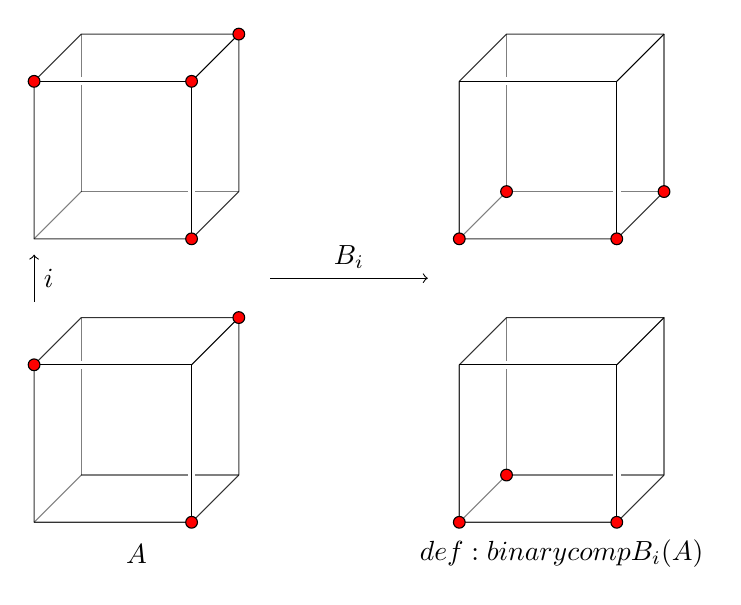
\begin{tikzpicture}[scale=2]
    \begin{scope}[every node/.style={inner sep=0, minimum size=0, outer sep=0}, mymark/.style={inner sep=1.5pt, draw=black, fill=red, circle}, over/.style={white, line width=1.2pt, double distance=0.4pt, shorten < = 1pt}]
      \begin{scope}
        \node (A) at (0,0) {};
        \node (B) at (1,0) {};
        \node (C) at (1,1) {};
        \node (D) at (0,1) {};
        \node (E) at (0.3,0.3) {};
        \node (F) at (1.3,0.3) {};
        \node (G) at (1.3,1.3) {};
        \node (H) at (0.3,1.3) {};
        \foreach \x in {A,F,H} {\draw [opacity=0.5] (E) -- (\x);};
        \foreach \x in {B,D,G} {\draw [over] (C) -- (\x); \draw (C) -- (\x);};
        \draw [line cap=round, opacity=0.8] (A) -- (B) -- (F) -- (G) -- (H) -- (D) -- (A);
        \foreach \x in {B,C,D,G} {\node [mymark] at (\x) {};}
      \end{scope}
      \begin{scope}[yshift=-1.8cm]
        \node (A) at (0,0) {};
        \node (B) at (1,0) {};
        \node (C) at (1,1) {};
        \node (D) at (0,1) {};
        \node (E) at (0.3,0.3) {};
        \node (F) at (1.3,0.3) {};
        \node (G) at (1.3,1.3) {};
        \node (H) at (0.3,1.3) {};
        \foreach \x in {A,F,H} {\draw [opacity=0.5] (E) -- (\x);};
        \foreach \x in {B,D,G} {\draw [over] (C) -- (\x); \draw (C) -- (\x);};
        \draw [line cap=round, opacity=0.8] (A) -- (B) -- (F) -- (G) -- (H) -- (D) -- (A);
        \foreach \x in {B,D,G} {\node [mymark] at (\x) {};}
      \end{scope}
      \begin{scope}[xshift=2.7cm]
        \node (A) at (0,0) {};
        \node (B) at (1,0) {};
        \node (C) at (1,1) {};
        \node (D) at (0,1) {};
        \node (E) at (0.3,0.3) {};
        \node (F) at (1.3,0.3) {};
        \node (G) at (1.3,1.3) {};
        \node (H) at (0.3,1.3) {};
        \foreach \x in {A,F,H} {\draw [opacity=0.5] (E) -- (\x);};
        \foreach \x in {B,D,G} {\draw [over] (C) -- (\x); \draw (C) -- (\x);};
        \draw [line cap=round, opacity=0.8] (A) -- (B) -- (F) -- (G) -- (H) -- (D) -- (A);
        \foreach \x in {A,B,E,F} {\node [mymark] at (\x) {};}
      \end{scope}
      \begin{scope}[xshift=2.7cm, yshift=-1.8cm]
        \node (A) at (0,0) {};
        \node (B) at (1,0) {};
        \node (C) at (1,1) {};
        \node (D) at (0,1) {};
        \node (E) at (0.3,0.3) {};
        \node (F) at (1.3,0.3) {};
        \node (G) at (1.3,1.3) {};
        \node (H) at (0.3,1.3) {};
        \foreach \x in {A,F,H} {\draw [opacity=0.5] (E) -- (\x);};
        \foreach \x in {B,D,G} {\draw [over] (C) -- (\x); \draw (C) -- (\x);};
        \draw [line cap=round, opacity=0.8] (A) -- (B) -- (F) -- (G) -- (H) -- (D) -- (A);
        \foreach \x in {A,B,E} {\node [mymark] at (\x) {};}
      \end{scope}
    \end{scope}
    \draw [->] (0, -0.4) -- (0, -0.1) node [right, midway] {$i$};
    \node at (0.65,-2) {$A$};
    \node at (3.35,-2) {$\hyperlink{def:binarycomp}{B_i(A)}$};
    \draw [->] (1.5, -0.25) -- (2.5, -0.25) node [above, midway] {$B_i$};
  \end{tikzpicture}
\end{center}
\begin{nthm}[Edge-isoperimetric inequality in the cube]\label{thm:2.8}
  Let $A \subset \hyperlink{def:qn}{Q_n}$, and let $C$ be the initial segment of the \hyperlink{def:binary}{binary ordering} with $|C| = |A|$. Then $|\hyperlink{def:ebound}{\partial} A| \geq |\partial C|$.
  In particular, if $|A|=2^k$ then $|\partial A| \geq 2^k (n-k)$.
\end{nthm}
\begin{remark}
  Sometimes called the theorem of Harper, Lindsey, Bernstein and Hart.
\end{remark}
\begin{proof}
  Induction on $n$: $n=1$ is immediate.
  Given $A \subset \hyperlink{def:qn}{Q_n}$ for $n > 1$ and $1 \leq i \leq n$: \textbf{Claim} $|\hyperlink{def:ebound}{\partial} \hyperlink{def:binarycomp}{B_i}(A)| \leq |\partial A|$.

  \textbf{Proof of claim:} Write $B$ for $B_i(A)$.
  We have
  \begin{align*}
    |\partial A| &= |\partial(A_-)| + |\partial(A_+)| + |A_i \sym A_+| \\
    |\partial B| &= |\partial(B_-)| + |\partial(B_+)| + |B_i \sym B_+|.
  \end{align*}
  Now, $|\partial (B_-)| \leq |\partial (A_-)|$ and $|\partial(B_+)| \leq |\partial(A_+)|$ by induction.
  Also, $|A_-| = |B_-|$, $|A_+| = |B_+|$ and $B_-, B_+$ nested (as both initial segments of \hyperlink{def:binary}{binary}).
  Whence $|B_- \sym B_+| \leq |A_i \sym A_+|$.
  Among all $B \subset Q_n$ with $|B| = |A|$ and $|\partial B| \leq |\partial A|$, choose one with
  \begin{equation*}\sum_{x \in B} (\text{position of $x$ in binary order})\end{equation*}
  minimal, completing the claim. $\blacksquare$

  Then $B$ is \hyperlink{def:binarycomp}{$i$-binary compressed} $\forall i$ by claim.
  This $B$ need not be an initial segment of binary, e.g.\
  \begin{center}
    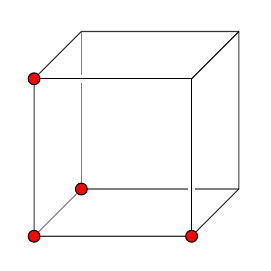
\begin{tikzpicture}[scale=2]
      \begin{scope}[every node/.style={inner sep=0, minimum size=0, outer sep=0}, mymark/.style={inner sep=1.5pt, draw=black, fill=red, circle}, over/.style={white, line width=1.2pt, double distance=0.4pt, shorten < = 1pt}]
        \node (A) at (0,0) {};
        \node (B) at (1,0) {};
        \node (C) at (1,1) {};
        \node (D) at (0,1) {};
        \node (E) at (0.3,0.3) {};
        \node (F) at (1.3,0.3) {};
        \node (G) at (1.3,1.3) {};
        \node (H) at (0.3,1.3) {};
        \foreach \x in {A,F,H} {\draw [opacity=0.5] (E) -- (\x);};
        \foreach \x in {B,D,G} {\draw [over] (C) -- (\x); \draw (C) -- (\x);};
        \draw [line cap=round, opacity=0.8] (A) -- (B) -- (F) -- (G) -- (H) -- (D) -- (A);
        \foreach \x in {A,B,D,E} {\node [mymark] at (\x) {};}
    \end{scope}
    \end{tikzpicture}
  \end{center}

  However, claim: If $B< Q_n$ is $i$-binary compressed $\forall i$ but not an initial segment of binary, then
  \begin{equation*}B = \mathcal{P}([n-1]) \cup \{n\} - \{123\dotsm(n-1)\}.\end{equation*}
  (Bottom half with last point removed, first point of top half added).
  \begin{center}
    \begin{tikzpicture}[scale=2]
      \fill [bred!40] (0,0) -- (1,0) -- (1,0.85) arc [start angle=-90, end angle=-180, radius=1.5mm] -- (0,1);
      \fill [bred!40] (0.15,1.5) arc [start angle=0, end angle=90, radius=1.5mm] -- (0,1.5);
      \draw (0,0) rectangle (1,1);
      \draw (0,1.5) rectangle (1,2.5);
      \draw [->] (-0.2,0.9) to node[midway, left] {$n$} (-0.2,1.6);
      \node [right] at (1.1, 0.5) {$Q_{n-1}$};
      \node [right] at (1.1, 2) {$Q_{n-1}$};
    \end{tikzpicture}
  \end{center}
  Then done, as clearly $|\partial B| \geq |\partial C|$.

  Proof of claim:
  Have some $x < y$ with $x \notin B$ and $y \in B$.
  Then $\forall i$, cannot have $i \notin x,y$ and cannot have $i \in x,y$ as $B_i(B) = B$.
  So $x = y^c$.
  Thus for each $y \in B$, there is at most 1 $x < y$ with $x \notin B$ (namely $x^c$), and for each $x \notin B$, there is at most one $y > x$ with $y \in B$ (namely $y^c$).
  Hence $B = \set{z | z \leq y} - \{x\}$ where $x$ is the immediate predecessor of $y$ and $x = y^c$.
  Hence $y = \{n\}$.
\end{proof}
\begin{remark}
  In the proofs of \cref{thm:harper1} and \cref{thm:2.8}, vital that the extremal sets in dimension $n-1$ were nested, i.e.\ were the initial segments of some ordering.
\end{remark}

\begin{defi}[Isoperimetric number]\hypertarget{def:i}
  The \marginnote{\emph{Lecture 11}}\named{isoperimetric number} of a graph $G$ is
  \begin{equation*}
    i(G) \coloneqq \Set{\frac{\lvert\partial A\rvert}{\lvert A\rvert} | A \subset G, |A| \leq \frac{1}{2}|G|}.
  \end{equation*}
  `How small can the average out-degree be?'
\end{defi}
\begin{center}
  \begin{tikzpicture}
    \begin{scope}
      \coordinate (0) at (-1,-0.1);
      \coordinate (1) at (-0.7,0.1);
      \coordinate (2) at (-0.5, 0);
      \coordinate (3) at (-0.3,0.2);
      \coordinate (4) at (0,-0.15);
      \coordinate (5) at (0.1,0);
      \coordinate (6) at (0.3,0.1);
      \coordinate (7) at (0.4,-0.2);
      \coordinate (8) at (0.6,0);
      \clip (0,0) circle [x radius=1cm, y radius=1.5cm];
      \draw [bred, fill=bred!40] plot coordinates {(0) (1) (2) (3) (4) (5) (6) (7) (8) (1,-0.1) (1,-1.6) (-1,-1.6)};
      \foreach \x in {1,3,6,8} {
        \draw [bgreen] (\x) -- ++(110+rand*20:0.25);
        \draw [bgreen] (\x) -- ++(60+rand*20:0.25);
      }
      \draw [bgreen] (5) -- ++(100:0.2);
      \draw [bgreen] (2) -- ++(90:0.2);
      \draw [bgreen] (-0.15,0.025) -- ++(80:0.2);
    \end{scope}
    \draw (0,0) circle [x radius=1cm, y radius=1.5cm];
    \node [bred!70!black] at (0,-1) {$A$};
  \end{tikzpicture}
\end{center}
\begin{ncor}\label{cor:2.9}
  $\hyperlink{def:i}{i(Q_n)}=1$.
\end{ncor}

\begin{center}
  \begin{tikzpicture}[scale=2]
    \begin{scope}[every node/.style={inner sep=0, minimum size=0, outer sep=0}, mymark/.style={inner sep=1.5pt, draw=black, fill=red, circle}, over/.style={white, line width=1.2pt, double distance=0.4pt, shorten < = 1pt}, mymarkline/.style={line cap=round, ultra thick, bgreen, opacity=0.5}]
      \begin{scope}
        \node (A) at (0,0) {};
        \node (B) at (1,0) {};
        \node (C) at (1,1) {};
        \node (D) at (0,1) {};
        \node (E) at (0.3,0.3) {};
        \node (F) at (1.3,0.3) {};
        \node (G) at (1.3,1.3) {};
        \node (H) at (0.3,1.3) {};
        \fill [bred!40] (A) -- (B) -- (1.3,0.3) -- (0.3,0.3) -- (0,0);
        \foreach \x in {A,F,H} {\draw [opacity=0.5] (E) -- (\x);};
        \draw [mymarkline] (E) -- (H);
        \foreach \x in {D,G} {\draw [over] (C) -- (\x); \draw (C) -- (\x);};
        \draw (C) -- (B);
        \draw [mymarkline] (G) -- (F);
        \draw [line cap=round, opacity=0.8] (A) -- (B) -- (F) -- (G) -- (H) -- (D) -- (A);
        \draw [mymarkline] (B) -- (C);
        \draw [mymarkline] (A) -- (D);
      \end{scope}
  \end{scope}
  \node [bred!70!black] at (0.65,0.15) {$A$};
  \end{tikzpicture}
\end{center}

\begin{proof}
  The set $A = \mathcal{P}(\hyperlink{def:ints}{[n-1]})$ shows $\hyperlink{def:i}{i(Q_n)}\leq1$.
  To show $i(Q_n) \geq 1$, sufficient to show (by \cref{thm:2.8}) that if $C$ is an initial segment of binary with $|C| \leq 2^{k-1}$ then $|\partial C| \geq |C|$.
  \begin{center}
    \begin{tikzpicture}[scale=2]
      \begin{scope}[every node/.style={inner sep=0, minimum size=0, outer sep=0}, mymark/.style={inner sep=1.5pt, draw=black, fill=red, circle}, over/.style={white, line width=1.2pt, double distance=0.4pt, shorten < = 1pt}, mymarkline/.style={->, bgreen, opacity=0.9}]
        \begin{scope}
          \node (A) at (0,0) {};
          \node (B) at (1,0) {};
          \node (C) at (1,1) {};
          \node (D) at (0,1) {};
          \node (E) at (0.3,0.3) {};
          \node (F) at (1.3,0.3) {};
          \node (G) at (1.3,1.3) {};
          \node (H) at (0.3,1.3) {};
          %\fill [bred!40] (A) -- (B) -- (1.3,0.3) -- (0.3,0.3) -- (0,0);
          \draw [bred, fill=bred!40] decorate[decoration={random steps,segment length=2pt,amplitude=1pt}] {(0.6,0.3) -- (0.95,0)} -- (0,0) -- (0.3,0.3) -- (0.6,0.3);
          \foreach \x in {A,F,H} {\draw [opacity=0.5] (E) -- (\x);};
          \draw [mymarkline] (E) -- (0.3,0.9);
          \draw [mymarkline] (0.6,0.3) -- (0.6,0.9);
          \foreach \x in {D,G} {\draw [over] (C) -- (\x); \draw (C) -- (\x);};
          \draw (C) -- (B);
          %\draw [mymarkline] (G) -- (F);
          \draw [line cap=round, opacity=0.8] (A) -- (B) -- (F) -- (G) -- (H) -- (D) -- (A);
          \draw [mymarkline] (0.95,0) -- (0.95,0.6);
          \draw [mymarkline] (A) -- (0,0.6);
        \end{scope}
      \end{scope}
    \node [bred!70!black] at (0.45,0.15) {$C$};
    \end{tikzpicture}
  \end{center}
  But this is clear because $C \subset \mathcal{P}([n-1])$.
\end{proof}

\subsection{Inequalities in the grid}
\begin{defi}[Grid]\hypertarget{def:grid}
  The \named{grid} is the graph on vertex-set $[k]^n = \{1,2,\dotsc,k\}^n$ in which $(x_1, \dotsc, x_n)$ joined to $(y_1, \dotsc, y_n)$ if for some $i$, have $|x_i - y_i| = 1$ and $x_j = y_j \quad \forall j \neq i$ (`$\ell^1$-distance').
\end{defi}
\begin{center}
  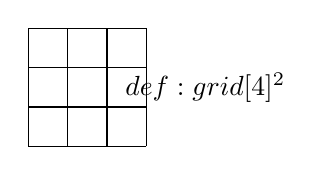
\begin{tikzpicture}[scale=0.5]
    \draw (0,0) grid (3,3);
    \node at (4.5,1.5) {$\hyperlink{def:grid}{[4]^2}$};
  \end{tikzpicture}
\end{center}
For $k=2$, this is the \hyperlink{def:qn}{discrete cube $Q_n$}.

Do \cref{thm:harper1} and \cref{thm:2.8} have analogues in \hyperlink{def:grid}{$[k]^n$}?
What is the best \hyperlink{def:boundary}{vertex-boundary}? Take $[k]^2$ as an example:
\begin{center}
  \begin{tikzpicture}[scale=2]
    \begin{scope}
    \draw [bred, fill=bred!40] (0,0) -- (0.7,0) -- (0,0.7);
    \draw (0,0) rectangle (1,1);
    \draw [decorate, decoration={brace, amplitude=2mm}, xshift=-0.5mm] (0,0) -- node [midway, left, xshift=-2mm] {$d$} (0,0.7);
    \node [right] at (1.1,0.5) {has $|\hyperlink{def:boundary}{b(A)}| \sim d \sim \sqrt{2|A|}$};
    \end{scope}
    \begin{scope}[yshift=-1.4cm]
      \draw [bred, fill=bred!40] (0,0) -- (0.4,0) -- (0.4,0.4) -- (0,0.4);
      \draw (0,0) rectangle (1,1);
      \draw [decorate, decoration={brace, amplitude=2mm}, xshift=-0.5mm] (0,0) -- node [midway, left, xshift=-2mm] {$d$} (0,0.4);
      \node [right] at (1.1,0.5) {has $|\hyperlink{def:boundary}{b(A)}| \sim 2d \sim 2\sqrt{|A|}$};
    \end{scope}
  \end{tikzpicture}
\end{center}

This suggests that sets of the form $ \set{x | \lvert x \rvert \leq r} $ are best.

What about sizes in between?
For given $|x|$, we'd `keep $x_1$ big'
\begin{defi}[Simplicial ordering]\hypertarget{def:simplic}
  We define the \index{simplicial ordering} on $[k]^n$ by setting $x<y$ if either $|x| < |y|$ or $|x| = |y|$ and $x_i > y_i$, where $i = \min\set{j | x_j \neq y_j}$.
  Note: for $k=2$ this agrees with our \hyperlink{def:simplicial}{previous definition}.
\end{defi}
\begin{eg}\leavevmode
  \begin{itemize}
    \item On $[3]^2$, our ordering is
      \begin{equation*}
        (1,1),(2,1),(1,2),(3,1),(2,2),(1,3),(3,2),(2,3),(3,3).
      \end{equation*}
      \begin{center}
        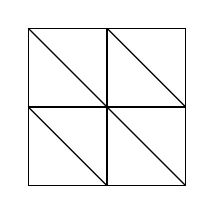
\begin{tikzpicture}
          \draw (0,0) grid (2,2);
          \draw (1,0) -- (0,1);
          \draw (2,0) -- (0,2);
          \draw (2,1) -- (1,2);
        \end{tikzpicture}
      \end{center}
    \item On $[4]^3$, we get
      \begin{equation*}
        111,211,121,112,311,221,212,131,122,113,411,321,\dotsc
      \end{equation*}
  \end{itemize}
\end{eg}
\begin{aim}
  Initial segments of \hyperlink{def:simplic}{simplicial} minimise \hyperlink{def:neighbourhood}{neighbourhood}.
  In particular,
  \begin{equation*}
    |A| = |\set{x | |x|\leq r}| \implies |\hyperlink{def:neighbourhood}{N(A)}| \geq |\set{x | |x| \leq r+1}|.
  \end{equation*}
\end{aim}
\begin{defi}[Sections]\index{$i$-section}
  \hypertarget{def:sections}For $A \subset [k]^n$ and $1 \leq i \leq n$, the \textbf{$i$-sections} of $A$ are the sets $A_1, \dotsc, A_k$ (or $A_1^{(i)}, \dotsc, A_k^{(i)}$) in $[k]^{n-1}$ given by
  \begin{equation*}
    A_t = \set{(x_1, \dotsc, x_{n-1}) \in [k]^{n-1} | (x_1, x_2, \dotsc, x_{i-1}, t, x_i, x_{i+1}, \dotsc, x_n) \in A} \quad \forall 1 \leq t \leq k
  \end{equation*}
\end{defi}
% TODO: picture
\begin{defi}[$i$-compression]\hypertarget{def:icomp2}
  The \textbf{$i$-compression} $C_i(A) \subseteq [k]^n$ is defined by giving its \hyperlink{def:sections}{$i$-sections}:
  \begin{equation*}
    C_i(A)_t = \text{first $|A_t|$ points in \hyperlink{def:simplic}{simplicial order} on }[k]^{n-1}.
  \end{equation*}
\end{defi}
Certainly $|C_i(A)| \leq |A|$.
Say $A$ is \textbf{$i$-compressed} if $C_i(A) = A$.
\begin{nthm}[Vertex-isoperimetric inequality in the grid]
  Let $A \subseteq [k]^n$ and let $C$ be the initial segment of the simplicial order on $[k]^n$ with $|C| = |A|$.
  Then $|N(A)| \geq |N(C)|$. In particular, if $|A| \geq |\set{x | |x|\leq r}|$ then $|N(A)| \geq |\set{x | |x| \leq r+1}|$
\end{nthm}
\begin{proof}
  Induction on $n$:
  For $n=1$, if $A \subset [k]^1$ with $A \neq 0, [k]^1$ then $|N(A)| \geq |A|+1 = |N(C)|$, as required.

  Given $A \subset [k]^n$ (for $n > 1$) and $1 \leq t \leq n$,
  \textbf{claim} $|N(C_t(A))| \leq |N(A)|$.

  \textbf{Proof of claim:}
  For $1 \leq t \leq k$,
  \begin{equation*}
    N(A)_t = N(A_t) \cup A_{t-1} \cup A_{t+1} % TODO: from level t, from below, from above
  \end{equation*}
  (where $A_0 = A_{k+1}=\emptyset$) and similarly
  \begin{equation*}
    N(B)_t = N(B_t) \cup B_{t-1} \cup B_{t+1}.
  \end{equation*}
  Now, $|B_{t-1}| = |A_{t-1}|$ and $|B_{t+1}| = |A_{t+1}|$.
  Also, $|N(B_t)| \leq |N(A_t)|$ (induction).

  But the sets $B_{t-1}$, $B_{t+1}$, $N(B_t)$ are nested (as each is an initial segment), so $|N(B)_t| \leq |N(A)_t|$.
  This holds for each $1 \leq t \leq k$. $\blacksquare$

  Among all $B \subseteq [k]^n$ with $|B| = |A|$ and $|N(B)| \leq |N(A)|$, choose one with minimal
  \begin{equation*}
    \sum_{x \in B} (\text{position of $x$ in simplicial}).
  \end{equation*}
  Then $B$ is $i$-compressed $\forall i$ (else $C_i(B)$ contradicts our discussion of $B$).

  \marginnote{\emph{Lecture 12}}We want to show $N(B) \geq N(C)$.
  \begin{itemize}
    \item \textbf{Case 1}: $n=2$.
      $B$ is $i$-compressed $\forall i$ if and only if $B$ is a \textbf{down-set} (if $x_i \leq y_i \; \forall i$ and $y \in B)$ then $x \in B$). That is, `going down or left, we stay in $B$'.
      Suppose $B \neq C$.
      Let
      \begin{align*}
        r &= \min \set{\lvert x \rvert | x \notin B} \\
        s &= \max \set{\lvert x \rvert | x \in B}.
      \end{align*}
      We must have $r \leq s$, since $r > s \Rightarrow B = C$, as $B$ would be an exact ball.

      If $r=s$, have
      \begin{equation*}
        \set{x : |x| \leq r-1} \subset B \subset \set{x | |x|\leq r},
      \end{equation*}
      so clearly $|N(B)| \geq |N(C)|$.

      If $r < s$, we cannot have $\set{x | |x| = r}$ disjoint from $B$ (as $B$ is a down-set and $\exists x \in B$ with $|x| = s$).
      Similarly cannot have $\set{x | |x| = s} \subset B$ (as $B$ a down-set and $\exists x \notin B, |x| = r$).
      So $\exists x,x'$ on level $r$ with $x \notin B, x' \in B$ and $x' = x \pm (e_1 - e_2)$, and $\exists y,y'$ on level $s$ with $y \in B$, $y' \notin B$ and $y' = y \pm (e_1 - e_2)$.

      Now let $B' = B \cup \{x\} - \{y\}$. Then $N(B') \leq N(B)$ (we lose $\geq 1$ point from level $s+1$ and gain $\leq 1$ point from level $r+1$), contradicting choice of $B$.
    \item \textbf{Case 2}: $n \geq 3$.
      If $x \in B$ then must have $x-e_n+e_i \in B$ (for any $1 \leq i \leq n-1$, $x_n > 1$, $x_i \leq k$), because $B$ is $j$-compressed, any $j \neq n,i$ (as $n \geq 3$).
      So $N(B_t) \subset B_{t-1}$.
      We had $N(B)_t = N(B_t) \cup B_{t-1} \cup B_{t+1}$, so $N(B)_t = B_{t-1}$.
      Thus

      \begin{equation*}
        |N(B)| = |B_{k-1}| + |B_{k-2}| + \dotsb + |B_1| + |N(B_1)| = |B| - |B_k| + |N(B_1)|
      \end{equation*}
      where $B_1$ is in level 2, and $N(B_1)$ is in level 1.
      Similarly,
      \begin{equation*}
        |N(C)| = |C| - |C_k| + |N(C_1)|.
      \end{equation*}
      Thus it is sufficient to show that $|B_k| \leq |C_k|$ and $|B_1| \geq |C_1|$.
      Focus on the former first:
      Define  $D \subset [k]^n$ by
      \begin{align*}
        D_k &= B_k \\
        D_t &= N(D_{t+1}), \quad t = k-1, k-2, \dotsc, 1
      \end{align*}
      Then $D$ is an initial segment of simplicial, and $D \subset B$, so $|D| \leq |B| = |C|$, whence $D \subset C$ (as $D,C$ nested as initial segments of simplicial).
      Hence $D_k \subset C_k$.

      Now aim to show $|B_1| \geq |C_1|$:
      Define $E \subset [k]^n$ by
      \begin{align*}
        E_1 &= B_1 \\
        E_t &= \set{x \in [k]^{n-1} | N(\{x\}) \subset E_{t-1}}, \quad t=2,3,\dotsc,k.
      \end{align*}
      Then $E$ is an initial segment of simplicial and $E \supset B$, so $|E| \geq |B| = |C|$, whence $E \supset C$ (as $E,C$ nested). Hence $E_1 \supset C_1$.
      This completes the claim, and thus completes the induction. \qedhere
  \end{itemize}
\end{proof}
\begin{ncor}\label{cor:2.11}
  Let $A \subset [k]^n$ with $|A| = |\set{x | |x| \leq r}|$. Then $|A_{(t)}| \geq |\set{x | |x| \leq r + t}$.
\end{ncor}
\begin{proof}
  Induction on $t$.
\end{proof}
\begin{remark}
  Can check from this that, for fixed $k$, the sequence $[k]^1, [k]^2, [k]^3, \dotsc$ is a \hyperlink{def:levyfam}{normal L\'evy family}.
\end{remark}
\subsection{Edge-isoperimetric inequalities in the grid}
We aim to minimise $|\partial A|$ in $[k]^m$.
For example, in $[k]^2$:
\begin{center}
  pictures
\end{center}
% TODO: draw some pictures
This suggests squares are best.
But,
\begin{center}
  more pictures
\end{center}
% TODO: draw some more pictures
so have `phase transitions' at $|A| = \frac{k^2}{4}$ and $|A| = \frac{3k^2}{4}$.
The extremal sets are not nested! (So cannot compress, $\nexists$ an ordering, etc.)

In $[k]^3$:
\begin{center}
  equation
\end{center}

Similarly in higher dimensions.
This has been proved: `edge-isoperimetric inequality in the grid'.

Very few isoperimetric inequalities are known exactly or asymptotically.
\clearpage
\section{Projections}
`If a set has small projections, must it be small?'
\begin{center}
  \begin{tikzpicture}
    \draw [->] (-0.1,0) -- (3.1,0);
    \draw [->] (0,-0.1) -- (0,3.1);
    \draw [very thin] (2.8,2.528) -- (0,2.528);
    \draw [very thin] (2.8,0.4) -- (0,0.4);
    \draw [very thin] (0.6,0) -- (0.6,2.8);
    \draw [very thin] (2.605,0) -- (2.605,2.8);
    \draw [xshift=1.6cm,yshift=1.6cm, bred, fill=bred!40] plot [smooth cycle, tension=0.7] coordinates {(0:1) (45:1.15) (90:0.9) (135:1.05) (180:1) (-135:1) (-90:1.2) (-45:1.1)};
    \node [bred!70!black] at (1.6,1.6) {$A$};
    \node [below] at (0.6,0) {$4$};
    \node [below] at (2.605,0) {$10$};
    \node [left] at (0,0.4) {$2$};
    \node [left] at (0,2.528) {$13$};
    \node [right] at (3,1.6) {$|A| \leq 6 \cdot 11$};
  \end{tikzpicture}
\end{center}
\begin{defi}[Projection]\hypertarget{def:proj}
  Let\marginnote{\emph{Lecture 13}} $A \subset \mathcal{P}(X)$. For $Y \subset X$ the \named{projection} or \named{trace} of $A$ on $Y$ is
  \begin{equation*}A \mid Y \coloneqq \set{x \cap Y | x \in A}.\end{equation*}
`Project $A$ onto coordinates corresponding to $Y$'.
\end{defi}
\begin{eg}
  If $A = \{14,25,26,127,128\}$. Then $A \mid \{1,2\} = \{1,2,12\}$, so $A \mid Y \subset \mathcal{P}(Y)$.
\end{eg}
\begin{defi}[Cover]\hypertarget{def:tr}
  Say $A$ \textbf{covers} or \textbf{shatters} $Y$ if $\hyperlink{def:proj}{A \mid Y} = \mathcal{P}(Y)$.
  The \textbf{trace number} or \textbf{VC-dimension} of $A$ is
  \begin{equation*}
    \tr A \coloneqq \max\{|Y| : A \text{ shatters } Y\}.
  \end{equation*}
\end{defi}
Given $|A|$, how small can $\hyperlink{def:tr}{\tr} A$ be?
Equivalently, if $\tr A < k$ ($A$ does not shatter any $k$-set), how large can $A$ be?

Trivially, must have
\begin{equation*}
  |A| \leq \left(1 - \frac{1}{2^k}\right) 2^n
\end{equation*}
else $A$ \hyperlink{def:tr}{shatters} every \hyperlink{def:superr}{$k$-set}.
Could take $A = X^{(<k)}$ - no $k$-set $Y$ is shattered, as $Y \notin A \hyperlink{def:proj}{\mid} Y$.

\begin{aim}
  This is best.
\end{aim}
\begin{remark}
  Very striking, as from each $k$-\hyperlink{def:proj}{projection} having size $\leq (1 - \frac{1}{2^k}) \cdot \text{total}$, we are getting a very small (polynomial in $n$) bound on $|A|$.
\end{remark}

\begin{idea}
  \hypertarget{def:downset}Trivial that $|A| \leq |X^{(<k)}|$ if $A$ is a \textbf{down-set} (if $x \in A$ and $y \subset x$ then $y \in A$).
  Indeed, must have $A \subset X^{(<k)}$, since if $A$ contains a set $x$ with $|x| \geq k$ then $A \mid x = \mathcal{P}(x)$.
  So `try to make $A$ into a down-set'.
\end{idea}

\begin{defi}[Down compression]
  \hypertarget{def:downcomp}For $A \subset \mathcal{P}(X)$ and $1 \leq i \leq n$, the $i$-\named{down-compression} of $A$ is defined as follows:
  For $x \in \mathcal{P}(X)$, set
  \begin{equation*}
    D_i(x) =
    \begin{cases}
      x & \text{if } i \notin x \\
      x-\{i\} & \text{if } i \in x \\
    \end{cases}
  \end{equation*}
  and set
  \begin{equation*}
    D_i(A) = \set{D_i(x) | x \in A} \cup \set{x \in A | D_i(x) \in A}
  \end{equation*}
  i.e.\ remove element $i$ where possible.
\end{defi}
\begin{nthm}[Sauer-Shelah Lemma]\label{thm:3.1}
  Let $A \subset \mathcal{P}(X)$ with $\hyperlink{def:tr}{\tr} A < k$. Then $|A| \leq |X^{(<k)}|$
\end{nthm}
\begin{proof}
  Given $1 \leq i \leq n$:
  Claim $\hyperlink{def:tr}{\tr}(\hyperlink{def:downcomp}{D_i(A)}) \leq \tr A$.

  Proof: Write $B = D_i(A)$.
  We'll show that if $B$ \hyperlink{def:tr}{shatters} $Y$ for some $Y$, then $A$ shatters $Y$.
  If $i \notin Y$ then $B \hyperlink{def:proj}{\mid} Y = A \mid Y$, so may assume $i \in Y$.
  Given $z \subset Y$ with $i \notin z$, we'll show $z, z \cup \{i\} \in A \mid Y$.
  Since $z \cup \{i\} \in B \mid Y$, we have $z \cup \{i\} \cup x \in B$, for some $x \subset X \setminus Y$.
  Hence $z \cup x$ and $z \cup \{i\} \cup x \in A$ (by definition of $D_i$)
  whence $z,z \cup \{i\} \in A \mid Y$, completing the claim.

  Now let $D = D_n(D_{n-1}(\dotsb D_1(A) \dotsb))$.
  Then $|D| = |A|$, $D$ is a \hyperlink{def:downset}{down-set}, and $\tr D \leq \tr A < k$.
  Thus $|D| \leq |X^{(<k)}|$.
\end{proof}
\begin{remark}
  We had $1$-dimensional compression.
\end{remark}
Have: if all $k$-dimensional \hyperlink{def:proj}{projections} have size $\leq 2^k - 1$, then $A$ small:
\begin{equation*}|A| \leq \sum_{i=0}^{k-1} \binom{n}{k}.\end{equation*}
What about other bounds?
For example, what if each $k$-dimensional projection is $\leq \frac{1}{2}$-sized: $|A \mid Y| \leq 2^{k-1}$?

\begin{defi}[Box]
  \hypertarget{def:box}A \named{box} or \named{brick} in $\mathbb{R}^n$ is a set of the form $[a_1, b_1] \times [a_2, b_2] \times \dotsb \times [a_n, b_n]$, where $a_i \leq b_i \; \forall i$.
\end{defi}
\begin{defi}[Body]\hypertarget{def:body}
  A \named{body} $S \subset \mathbb{R}^n$ is a finite union of \hyperlink{def:box}{bricks}.
  Write $|S|$ or $m(S)$ for the volume of $S$.
\end{defi}
\begin{remark}\leavevmode
  \begin{enumerate}[label=\arabic*.]
    \item Everything is unchanged if we only assume $S$ compact (or just bounded and measurable).
    \item For $A \subset \mathcal{P}(X) \leftrightarrow \{0,1\}^n$ we have corresponding \hyperlink{def:body}{body} $\hat{A} \subset \mathbb{R}^n$ with $m(\hat{A})= |A|$, namely:
      \begin{equation*}
        \hat{A} = \bigcup_{x \in A} [x_1,x_1+1] \times [x_2, x_2+1] \times \dotsb \times [x_n, x_n+1].
      \end{equation*}
      \begin{center}
        \begin{tikzpicture}[scale=1.5]
          \begin{scope}[every node/.style={inner sep=0, minimum size=0, outer sep=0}, mymark/.style={inner sep=1.5pt, draw=black, fill=red, circle}]
            \draw [bgreen, fill=bgreen!20!white, very thin] (0,0) -- (2,0) -- (2,1) -- (1,1) -- (1,2) -- (0,2) -- (0,0);
            \node [mymark] (A) at (0,0) {};
            \node [mymark] (B) at (1,0) {};
            \node [mymark] (C) at (0,1) {};
            \node (D) at (1,1) {};
            \draw (A) -- (B) -- (D) -- (C) -- (A);
            \node [left] at (-0.1,0.5) {${\color{bred!80!black}A} \subset Q_2$};
            \node [right] at (1.1,1.5) {${\color{bgreen!70!black}\hat{A}} \subset \mathbb{R}^2$};
        \end{scope}
        \end{tikzpicture}
      \end{center}
  \end{enumerate}
\end{remark}
\hypertarget{not:sy}For a body $S \subset \mathbb{R}^n$, and $Y \subseteq \{1,\dotsc,n\}$, write $S_Y$ for the projection of $S$ onto the subspace spanned by the $e_i,\ i \in Y$.
\begin{eg}
  For $S \subset \mathbb{R}^3$: $S_1$ is the projection of $S$ onto the $x$-axis, i.e.\
  \begin{equation*}
    S_1 = \set{x_1 | (x_1, x_2, x_3) \in S, \text{ some } x_2,x_3}
  \end{equation*}
  $S_{12}$ is the projection of $S$ onto the $xy$-plane.
  \begin{equation*}
    S_{12} = \set{(x_1,x_2) | (x_1, x_2, x_3) \in S, \text{ some } x_3}
  \end{equation*}
\end{eg}
\begin{center}
  \begin{tikzpicture}
    \draw [->] (0,0) -- (3,-1);
    \draw [->] (0,0) -- (0,4);
    \draw [->] (0,0) -- (4,0.5);
    \begin{scope}[transform canvas={yscale=0.8}, xshift=2cm, yshift=2.5cm]
      \shade [ball color = bred!40, opacity = 0.7] (0,0) circle (1cm);
    \end{scope}
    \draw (2,2) ellipse (1cm and 0.8cm);
    \draw (1,-0.1) -- (1,2);
    \draw (3,-0.1) -- (3,2);
    \draw (2,-0.1) ellipse (1cm and 0.2cm);
  \end{tikzpicture}
\end{center}
Do bounds on some of the $|S_Y|$ give bounds on $|S|$?

For \marginnote{\emph{Lecture 14}}example, for $S \subset \mathbb{R}^3$, we have both $|S| \leq |S_1| |S_2| \abs{S_3}$, as $S \subset S_1 \times S_2 \times S_3$, and $|S| \leq |S_{12}| |S_3|$, as $S \subset S_{12} \times S_3$.

But $|S_{12}| |S_{13}|$ does not bound $|S|$ - take for instance
\begin{equation*}
  S = \left[0, \frac{1}{N}\right] \times [0,N] \times [0,N].
\end{equation*}
How about $|S_{12}|,\ |S_{13}|,\ |S_{23}|$?
\begin{nprop}\label{prop:3.2}
  Let $S$ be a body in $\mathbb{R}^3$. Then $|S^2| \leq |S_{12}| |S_{13}| |S_{23}|$.
\end{nprop}
\begin{remark}\leavevmode
  \begin{enumerate}
    \item Can have equality, e.g.\ when $S$ is a \hyperlink{def:box}{brick}.
  \item \hypertarget{def:sectionr}For $S \subset \mathbb{R}^n$, the \named{section}\textbf{s} of $S$ are the sets $S(x) \subset \mathbb{R}^{n-1}$ (for $x \in \mathbb{R}$)
      given by
      \begin{equation*}
        S(x) = \set{(x_1, \dotsc, x_{n-1}) \in \mathbb{R}^{n-1} | (x_1, \dotsc, x_{n-1}, x) \in S}.
      \end{equation*}
  \end{enumerate}
\end{remark}
% TODO: picture
\begin{proof}
  Suppose first that every \hyperlink{def:sectionr}{section} of $S$ is a square: \begin{equation*}S(x) = [0, f(x)] \times [0, f(x)]\ \forall x.\end{equation*}
  Then $|S_{12}| = M^2$, where $M = \max f$.
  % TODO: picture
  Also,
  \begin{equation*}
    |S_{13}| = |S_{23}| = \int\!f(x) \, dx.
  \end{equation*}
  So want
  \begin{equation*}
    \left(\int\!f^2\right)^2 \leq M^2 \left(\int\!f\right)^2
  \end{equation*}
  i.e.\ $\int\!f^2 \leq M \int\!f$, which is true because $f(x)^2 \leq M f(x)$ for all $x$.

  For general $S$, define a body $T \subseteq \mathbb{R}^3$ by giving its sections:
  \begin{equation*}
    T(x) = \left[0, \sqrt{|S(x)|}\right] \times \left[0, \sqrt{|S(x)|}\right].
  \end{equation*}
  So $|T| = |S|$.
  Certainly have $|T_{12}| \leq |S_{12}|$ - since $|T_{12}| = \max|T(x)|$.
  Write
  \begin{equation*}
    \begin{aligned}
      g(x) &= |S(x)_1| \\
      h(x) &= |S(x)_2|
    \end{aligned}
    \qquad\text{so}\qquad
    |S(x)| \leq g(x) h(x).
  \end{equation*}
  % TODO: picture
  We have $|S_{13}| = \int g(x) \, dx$ and $|S_{23}| = \int h(x) \, dx$.
  Also,
  \begin{equation*}|T_{13}| = |T_{23}| = \int \sqrt{|S(x)|} \, dx \leq \int \sqrt{g(x) h(x)} \, dx.\end{equation*}
  So, we need $(\int\! \sqrt{gh})^2 \leq (\int\!g) (\int\!h)$, i.e.\ $\int\!\sqrt{gh} \leq (\int\!g)^{\frac{1}{2}} (\int\!h)^{\frac{1}{2}}$, which is Cauchy-Schwarz applied to $g^{\frac{1}{2}}, h^{\frac{1}{2}}$.
\end{proof}

\begin{defi}[Cover, uniform cover]\hypertarget{def:cover}
  Sets $Y_1, \dotsc, Y_r \subseteq \hyperlink{def:ints}{[n]}$ \named{cover} $[n]$ if $Y_1 \cup \dotsb \cup Y_r = [n]$.
  They are a \named{$k$-uniform cover} if each $i \in [n]$ belongs to exactly $k$ of $Y_1, \dotsc, Y_r$.
\end{defi}

\begin{eg}\leavevmode
  \begin{itemize}[label=--]
    \item $\{1\},\{2\},\{3\}$ is a \hyperlink{def:cover}{$1$-uniform cover} of $\hyperlink{def:ints}{[3]}$.
    \item $\{1\},\{2,3\}$ is a $1$-uniform cover of $[3]$.
    \item $\{1,2\},\{1,3\}$ is not a uniform cover of $[3]$.
    \item $\{1,2\},\{1,3\}, \{2,3\}$ is a $2$-uniform cover of $[3]$.
  \end{itemize}
\end{eg}
\begin{aim}
  $|S|^k \leq |S_{Y_1}| \dotsb |S_{Y_r}|$ where $Y_1, \dotsc, Y_r$ a \hyperlink{def:cover}{$k$-uniform cover} of $[n]$.
\end{aim}
Let $\mathcal{C} = {Y_1, \dotsc, Y_r}$ be a \hyperlink{def:cover}{$k$-uniform cover} of $[n]$.
This is a multiset, i.e.\ repetition allowed e.g.\ $\mathcal{C} = \{1,1,2,3,23\}$ is a $2$-uniform cover of $[3]$.
Let
\begin{equation*}
  \mathcal{C}_- = \set{Y \in \mathcal{C} | n \notin Y}, \qquad \mathcal{C}_+ = \set{Y - \{n\} | Y \in \mathcal{C}, n \in Y}.
\end{equation*}
So $|\mathcal{C}_+| = k$ and $\mathcal{C}_- \cup \mathcal{C}_+$ is a $k$-uniform cover of $[n-1]$.
Note that for a \hyperlink{def:body}{body} $S \subseteq \mathbb{R}^n$, if $n \notin Y$ then $|S_Y| \geq |S(x)_Y|\ \forall x$, e.g.\ $|S_1| \geq |S(x)_1|\ \forall x$ when $S \subseteq \mathbb{R}^3$.
Also, if $n \in Y$ then
\begin{equation*}
  |S_Y| = \int \left|S(x)_{Y-\{n\}}\right| \, dx
\end{equation*}
e.g.\ $|S_{13}| = \int |S(x)_1| \, dx.$

In the proof of \cref{prop:3.2}, we used Cauchy-Schwarz:
\begin{equation*}\int\!fg \leq \left(\int\!f^2\right)^\frac{1}{2}\, \left(\int\!g^2\right)^{\frac{1}{2}}.\end{equation*}
Here we'll need H\"older:
\begin{equation*}\int\!fg \leq \left(\int\!f^p\right)^\frac{1}{p} \left(\int\!g^q\right)^\frac{1}{q},\end{equation*}
where $\frac{1}{p} + \frac{1}{q} = 1$.
Iterating:
\begin{equation*}\int f_1 \dotsm f_k \leq \left(\int\!f_1^k\right)^\frac{1}{k} \dotsm \left(\int\!f_k^k\right)^\frac{1}{k}.\end{equation*}

\begin{nthm}[Uniform covers theorem]\label{thm:3.3}
  Let $S$ be a \hyperlink{def:body}{body} in $\mathbb{R}^n$, and let $\mathcal{C}$ be a \hyperlink{def:cover}{$k$-uniform cover} of $\hyperlink{def:ints}{[n]}$.
  Then $|S|^k \leq \prod_{Y \in \mathcal{C}} |S_Y|$.
\end{nthm}
\begin{proof}
  Induction on $n$: $n=1$ case works.
  Given $S \subset \mathbb{R}^n$ for $n \geq 2$:
  \begin{align*}
    |S| = \int\!|S(x)|\,dx &\leq \int \prod_{Y \in \mathcal{C}_-} |S(x)_Y|^{\frac 1 k}\prod_{Y \in \mathcal{C}_+} |S(x)_Y|^{\frac 1 k} \\
    \shortintertext{by induction, as $\mathcal{C}_- \cup \mathcal{C}_+$ a $k$-uniform cover of $[n-1]$}
                           &\leq \prod_{Y \in \mathcal{C}_-} |S_Y|^{\frac 1 k} \int \prod_{Y \in \mathcal{C}_+} \abs{S(x)_Y}^{\frac 1 k} \\
                           &\leq \prod_{Y \in \mathcal{C}_-} |S_Y|^{\frac 1 k} \prod_{Y \in \mathcal{C}_+} \left(\int \abs{S(x)_Y}\right)^{\frac 1 k} \\
                           &\leq \prod_{Y \in \mathcal{C}_-} |S_Y|^{\frac 1 k} \prod_{Y \in \mathcal{C}_+} \abs{S_{Y \cup \{n\}}}^{\frac 1 k} = \prod_{Y \in \mathcal{C}} |S_Y|^{\frac 1 k}. \qedhere
  \end{align*}
\end{proof}

\begin{ncor}[Loomis-Whitney theorem]\label{cor:3.4}
  \marginnote{\emph{Lecture 15}}Let $S$ be a \hyperlink{def:body}{body} in $\mathbb{R}^n$.
  Then
  \begin{equation*}
    |S|^{n-1} \leq \prod_{i=1}^n \abs{S_{\hyperlink{def:ints}{[n]} - \{i\}}}.
  \end{equation*}
\end{ncor}
\begin{remark}
  The $n=3$ case is \cref{prop:3.2}.
\end{remark}
\begin{proof}
  The sets $\hyperlink{def:ints}{[n]}- \{i\}$ for $1 \leq i \leq n$ form an \hyperlink{def:cover}{$(n-1)$-uniform cover} of $[n]$.
\end{proof}
\begin{ncor}\label{cor:3.5}
  Let $A \subset \mathcal{P}(\hyperlink{def:ints}{[n]})$ and let $\mathcal{C}$ be a \hyperlink{def:cover}{$k$-uniform cover} of $[n]$.
  Then
  \begin{equation*}|A|^k \leq \prod_{Y \in \mathcal{C}} |\hyperlink{def:proj}{A \mid Y}|.\end{equation*}
  In particular, if $|A \mid Y| \leq (2^{|Y|})^c$ $\forall Y \in \mathcal{C}$ then $|A| \leq (2^n)^c$.
\end{ncor}
\begin{proof}
  First part: identify $A$ with a body $\hat{A} \subseteq \mathbb{R}^n$.
  Second part:
  \begin{align*}
    |A|^k &\leq \prod_{Y \in \mathcal{C}} \abs{\hyperlink{def:proj}{A \mid Y}} \\
          &\leq \prod_{Y \in \mathcal{C}} (2^{|Y|})^c = (2^{\sum|Y|})^c \\
          &= 2^{k nc}. \qedhere
  \end{align*}
\end{proof}
\begin{aim}
  Bollob\'as-Thomason Box Theorem: For any $S \subset \mathbb{R}^n$, $\exists$ a \hyperlink{def:box}{box} $B$ with $|B| = |S|$ and $|\hyperlink{not:sy}{B_Y}| \leq |S_Y|$ $\forall Y \subseteq [n].$

  This looks way too strong to be true - e.g.\ it tells us that, to verify any proposed \hyperlink{def:proj}{projection} inequality, it suffices to check it on boxes.
\end{aim}
\begin{defi}[Irreducible cover]
  \hypertarget{def:irred}A \hyperlink{def:cover}{uniform cover} $\mathcal{C}$ of $[n]$ is \named{irreducible} if we cannot write $\mathcal{C} = \mathcal{C}' \cup \mathcal{C}''$ for some uniform covers $\mathcal{C}', \mathcal{C}''$.
\end{defi}
\begin{eg}
  If $n=3$, $\{12,13,23\}$ is \hyperlink{def:irred}{irreducible}, and $\{12,3,1,23\}$ is not.
\end{eg}
\begin{nlemma}
  There are only finitely many \hyperlink{def:irred}{irreducible covers} of $\hyperlink{def:ints}{[n]}$.
\end{nlemma}
\begin{proof}
  Suppose $\mathcal{C}_1, \mathcal{C}_2, \dotsc$ are \hyperlink{def:irred}{irreducible covers}.
  List $\mathcal{P}(\hyperlink{def:ints}{[n]})$ as $E_1, \dotsc, E_{2^n}$.
  There are subsequences $\mathcal{C}_{i_1}, \mathcal{C}_{i_2}, \dotsc$ on which the number of occurrences of $E_1$ is (not strictly) increasing.
  Find a subsequence of this on which the number of occurrences of $E_2$ is (not strictly) increasing.
  Repeating, we get $\mathcal{C}_{j_1}, \mathcal{C}_{j_2}, \dotsc$ on which $\forall E \subseteq [n]$, the number of occurrences of $E$ is increasing.
  But then $\mathcal{C}_{j_2}$ contains $\mathcal{C}_{j_1}$, so $C_{j_2}$ is not irreducible, a contradiction.
\end{proof}
\begin{nthm}[Bollob\'as-Thomason Box Theorem]\label{thm:3.7}
  Let $S \subset \mathbb{R}^n$ be a (non-empty) \hyperlink{def:body}{body}.
  Then $\exists$ a \hyperlink{def:box}{box} $B \subset \mathbb{R}^n$ with $|B| = |S|$ and $|\hyperlink{not:sy}{B_Y}| \leq |S_Y|\ \forall Y$.
\end{nthm}
\begin{proof}
  Without loss of generality, $|S| > 0$ and $n \geq 2$.
  Take real variables $x_Y$ for each $Y \subseteq \hyperlink{def:ints}{[n]}$ with $Y \neq \emptyset, [n]$.
  Consider the inequalities
  \begin{enumerate}[label=(\roman*)]
    \item $ 0 \leq x_Y \leq |\hyperlink{not:sy}{S_Y}|$ $\forall Y$.
    \item $x_Y \leq \prod_{i \in Y} x_i$ for each $|Y| \geq 2$
    \item $|S|^k \leq \prod_{Y \in \mathcal{C}} x_Y$, for each \hyperlink{def:irred}{irreducible} \hyperlink{def:cover}{$k$-uniform cover} $\mathcal{C}$ of $[n]$ and any $k$, with $\mathcal{C} \neq \{n\}$.
  \end{enumerate}
  (Our hope is to find such an $x_Y$ with $|S| = x_1 \dotsm x_n$ and $x_{12} = x_1 x_2$, etc - then the box is $[0, x_1] \times \dotsm \times [0, x_n]$.)

  Note that (iii) therefore holds for \emph{all} uniform covers, as it holds for irreducible ones.
  Now, $\exists$ a solution (e.g.\ set $x_Y = |S_Y|\ \forall Y$), and the solution set is compact, so $\exists$ a solution $(x_Y)$ with $\sum_Y x_Y$ minimal.
  Must have $x_Y > 0$ $\forall Y$ (as $|S| \leq x_Y x_{Y^c}$, by (iii)).

  \textbf{Claim:} For each $1 \leq i \leq n$, $x_i$ occurs on the right hand side of an inequality in (iii) in which equality holds.

  \textbf{Proof:} Must have $x_i$ on the right hand side of some inequality in which equality holds otherwise, we could decrease $x_i$ (as the set of inequalities is finite).
  It cannot be in (i) (as $x_i > 0$).
  If it is in (iii), we are done. If it is in (ii), we have $x_Y = \prod_{j \in Y} x_j$, for some $Y$ with $i \in Y$.

  But $x_Y$ must appear on right hand side of an equality (else could decrease it), which can only be in (iii).
  So we have a $k$-uniform cover $\mathcal{C}$ with $Y \in \mathcal{C}$ and $|S|^k = \prod_{z \in \mathcal{C}} x_z$.
  But then equality also holds for the cover $\mathcal{C}' = \mathcal{C} - \{Y\} \cup \set{\{j\} | j \in Y}$.
  Now just take an irreducible $\mathcal{C}'' \subset \mathcal{C}$ with $\{i\} \in \mathcal{C}''$. $\blacksquare$

  So, for each $i$, have a cover $\mathcal{C}_i$ with $\{i\} \in \mathcal{C}_i$ and equality holding in (iii).
  Put $\mathcal{C} = \mathcal{C}_1 \cup \dotsb \cup \mathcal{C}_n$. Then $\{i\} \in \mathcal{C}$ $\forall i$, and have equality for $\mathcal{C}$ in (iii).
  But $\mathcal{C} = \mathcal{C}' \cup \mathcal{C}''$ for some $\mathcal{C}''$, where $\mathcal{C}' = \set{\{i\} : 1 \leq i \leq n}$, hence have equality in (iii) for $\mathcal{C}'$, i.e.\ $|S| = x_1 \dotsm x_n$.
  Now for any $Y$ with $|Y| \geq 2$, must have $x_Y = \prod_{i \in Y} x_i$, because $Y,Y^c$ is a uniform cover, so that
  \begin{equation*}|S| \leq x_Y x_{Y^c} \leq \prod_{i \in Y} x_i \prod_{i \notin Y} x_i = x_1 \dotsm x_n = |S|.\qedhere\end{equation*}
\end{proof}

\subsection{Intersecting families of graphs}
So far, for \hyperlink{def:inter}{intersecting}\marginnote{\emph{Lecture 16}} families our objects lived in $\hyperlink{def:ints}{[n]}$.
What if the ground set has some structure?
For example, take the ground set as $[n]^{\hyperlink{def:superr}{(2)}}$, the edges of a graph on $[n]$, equivalently the subgraphs of $K_n$.
There are $2^{\binom n 2}$ possible graphs.

\begin{defi}[Intersecting]
  \hypertarget{def:hinter}Let $A \subset \mathcal{P}([n]^{(2)})$ be a family of graphs on $n$ vertices.
  For any fixed graph $H$, we say $A$ is \textbf{$H$-intersecting}\index{H-intersecting@$H$-intersecting}\index{intersecting} if $\forall G, G' \in A$, $G \cap G'$ contains a copy of $H$ (``$G \cap G' \supseteq H$'').
\end{defi}
For instance, take $H = P_1 =$ a single edge $=
  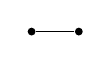
\begin{tikzpicture}[every node/.style=dot, scale=0.6]
    \node (A) at (0,0) {};
    \node (B) at (1,0) {};
    \draw (A) -- (B);
\end{tikzpicture}$

Then $A$ is \hyperlink{def:hinter}{$H$-intersecting} $\Rightarrow |A| \leq \frac{1}{2} 2^{\binom{n}{2}}$ (as we cannot have $G, G^c \subset A$), and can achieve this, e.g.\ $A = \set{G | 12 \in G}$.
(Indeed, for any non-empty $H$, we have $A$ $H$-intersecting $\Rightarrow |A| \leq \frac{1}{2} 2^{\binom n 2}$).

What about $H = P_2 =
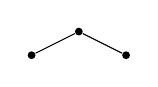
\begin{tikzpicture}[baseline=2pt, scale=0.3]
\node [dot] (A) at (0,0) {};
\node [dot] (B) at (2,1) {};
\node [dot] (C) at (4,0) {};
\draw [dot] (A) -- (B) -- (C);
\end{tikzpicture}$?
Obvious guess: the best is $A = \set{G | G \text{ contains } H_0}$, where $H_0$ is some fixed copy of $P_2$.
This has size $|A| = \frac{1}{4} 2^{\binom n 2}$.

But can do better, e.g.\ $A = \set{G | d_G(1) \geq \frac{n}{2} + 1}$, where $d_G(1)$ is the number of edges out of $1$.
This has size
\begin{equation*}
  |A| = 2^{\binom n 2} \left(\frac{1}{2} - \frac{c}{\sqrt n}\right) = \left(\frac{1}{2} - o(1)\right) 2^{\binom n 2}.
\end{equation*}
Similarly if $H$ is any star
\begin{center}
  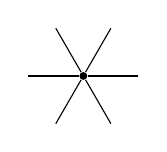
\begin{tikzpicture}
    \node [dot] (A) at (0,0) {};
    \foreach \x in {0,60,...,300} {
      \draw (A) -- (\x:0.7);
    }
  \end{tikzpicture}
\end{center}
we have \hyperlink{def:hinter}{$H$-intersecting} families of size $\left(\frac{1}{2} - o(1)\right) 2^{\binom n 2}$.

What about \hyperlink{def:hinter}{$\triangle$-intersecting}? Obvious guess is $|A| = \frac{1}{8} 2^{\binom n 2}$, achieved by
\begin{equation*}A = \set{G | G \supseteq \text{ fixed triangle}}.\end{equation*}
\begin{conjecture}[Simonovits-Sos]
  If $A$ is \hyperlink{def:hinter}{$\triangle$-intersecting} then $|A| \leq \frac{1}{8} 2^{\binom{n}{2}}.$
\end{conjecture}
\begin{nthm}\label{thm:3.8}
  Let $A \subset \mathcal{P}(\hyperlink{def:ints}{[n]}^{\hyperlink{def:superr}{(2)}})$ be \hyperlink{def:hinter}{$\triangle$-intersecting}.
  Then $|A| \leq \frac{1}{4} 2^{\binom n 2}$.
\end{nthm}
\begin{proof}
  Say $n$ even.
  Consider the \hyperlink{def:proj}{projection} of $A$ onto the edge-set $Y = B^{\hyperlink{def:superr}{(2)}} \cup (B^c)^{(2)}$, for any $B \subset \hyperlink{def:ints}{[n]}$ with $|B| = \frac{n}{2}$.
  Then $G, G' \in A \Rightarrow G \cap G'$ must meet $Y$ (because every triangle meets $Y$).
  % TODO: picture
  Then \hyperlink{def:proj}{$A \mid Y$} is an \hyperlink{def:inter}{intersecting} family of sets, so
  \begin{equation*}
    |A \mid Y| \leq \frac{1}{2} 2^{2 \binom{n/2}{2}} = 2^{2 \binom{n/2}{2} \cdot \left(1 - \frac{1}{2 \binom{n/2}{2}}\right)}.
  \end{equation*}
  But the $Y$ form a uniform cover of $[n]^{(2)}$ (as $B$ varies), so by \cref{cor:3.5} have
  \begin{equation*}
    |A| \leq 2^{\binom{n}{2} \cdot \left(1 - \frac{1}{2 \binom{n/2}{2}}\right)}.
  \end{equation*}
  So done if
  \begin{align*}
    \binom{n}{2} \frac{1}{2 \binom{n/2}{2}} \geq 2.
  \end{align*}
  But LHS = $\frac{n(n-1)}{2 \frac{n}{2} (\frac{n}{2}-1)} = \frac{n-1}{\frac{n}{2}-1} > 2$.

  For $n$ odd: same with $|B| = \frac{n-1}{2}$.
\end{proof}
The Simonovits-Sos conjecture was proved in 2010 (Ellis, Filmus, Friedgut).

\begin{defi}[Common]\hypertarget{def:common}
  Say $H$ \named{common} if
  \begin{equation*}
    \max \set{\abs{A} | A \subset \mathcal{P}(\hyperlink{def:ints}{[n]}^{\hyperlink{def:superr}{(2)}}) \text{ is \hyperlink{def:hinter}{$H$-intersecting}}} = \left(\frac{1}{2} - o(1)\right) 2^{\binom n 2}.
  \end{equation*}
\end{defi}
For instance, every star is \hyperlink{def:common}{common}, and $\triangle$ not common.
Any disjoint union of stars is also common, e.g.\ take $n$ very large, $k$ large and
\begin{equation*}
  A = \Set{G | \text{at least }\frac{n}{2} + 3\text{ of vertices $1,\dotsc,k$ have degree } \geq \frac{n}{2} + 5}.
\end{equation*}
\begin{center}
  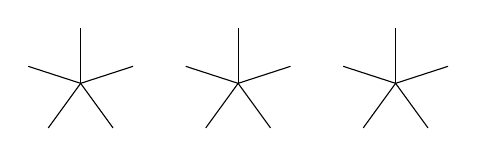
\begin{tikzpicture}
    \foreach \y in {0,2,4} {
      \foreach \x in {90,162,...,378} {
        \draw (\y,0) -- ++(\x:0.7);
      }
    }
  \end{tikzpicture}
\end{center}

Key question: Is $P_3$ \hyperlink{def:common}{common}? This is open.
%TODO: picture of P3
Easy fact: Every $G$ not a union of stars contains $\triangle$ of $P_3$.
So, if we know $P_3$ not common, we would know:

\begin{conjecture}[Alor's common graphs conjecture]
  $H$ \hyperlink{def:common}{common} $\iff H$ is a union of stars.
\end{conjecture}
But Christofides (2008) gave a \hyperlink{def:hinter}{$P_3$-intersecting} family with density $\frac{17}{128} > \frac{1}{8}$.
\printindex
\end{document}
